%%
%% This is file `elsarticle-template-harv.tex',
%% generated with the docstrip utility.
%%
%% The original source files were:
%%
%% elsarticle.dtx  (with options: `harvtemplate')
%%
%% Copyright 2007, 2008 Elsevier Ltd.
%%
%% This file is part of the 'Elsarticle Bundle'.
%% -------------------------------------------
%%
%% It may be distributed under the conditions of the LaTeX Project Public
%% License, either version 1.2 of this license or (at your option) any
%% later version.  The latest version of this license is in
%%    http://www.latex-project.org/lppl.txt
%% and version 1.2 or later is part of all distributions of LaTeX
%% version 1999/12/01 or later.
%%
%% The list of all files belonging to the 'Elsarticle Bundle' is
%% given in the file `manifest.txt'.
%%
%% Template article for Elsevier's document class `elsarticle'
%% with harvard style bibliographic references
%% SP 2008/03/01

%\documentclass[11pt]{elsart}
\documentclass[11pt,onecolumn]{elsart3p}
%\documentclass[final,1p,times,11pt]{elsarticle}

%% Use the option review to obtain double line spacing
%% \documentclass[authoryear,preprint,review,12pt]{elsarticle}

%% Use the options 1p,twocolumn; 3p; 3p,twocolumn; 5p; or 5p,twocolumn
%% for a journal layout:
%% \documentclass[final,1p,times]{elsarticle}
%% \documentclass[final,1p,times,twocolumn]{elsarticle}
%% \documentclass[final,3p,times]{elsarticle}
%% \documentclass[final,3p,times,twocolumn]{elsarticle}
%% \documentclass[final,5p,times]{elsarticle}
%% \documentclass[final,5p,times,twocolumn]{elsarticle}

%% if you use PostScript figures in your article
%% use the graphics package for simple commands
%% \usepackage{graphics}
%% or use the graphicx package for more complicated commands
\usepackage{epsf,graphicx}
%% or use the epsfig package if you prefer to use the old commands
%% \usepackage{epsfig}

%% The amssymb package provides various useful mathematical symbols
\usepackage{amssymb,amsmath}
%% The amsthm package provides extended theorem environments
%% \usepackage{amsthm}

%% The lineno packages adds line numbers. Start line numbering with
%% \begin{linenumbers}, end it with \end{linenumbers}. Or switch it on
%% for the whole article with \linenumbers.
%% \usepackage{lineno}

\usepackage{color}
\newcommand{\vermell}{\textcolor{red}}

\journal{}

\hyphenation{op-tical net-works semi-conduc-tor}

\newtheorem{theorem}{Theorem}
\newtheorem{lemma}{Lemma}
\newtheorem{observation}{Observation}
\newtheorem{property}{Property}

\newenvironment{proof}{\vspace{1ex}\noindent{\bf Proof}\hspace{0.5em}}
    {\hfill\qed\vspace{1ex}}


\usepackage[usenames,dvipsnames]{xcolor}
\newcommand{\added}{\textcolor{Green}}
\newcommand{\todecide}{\textcolor{Orchid}}
\newcommand{\todo}{\textcolor{red}}
\newcommand{\vell}{\textcolor{orange}}

\newcommand{\NACHO}[1]{\textcolor{red}{NACHO: #1}}
\newcommand{\TONI}[1]{\textcolor{red}{TONI: #1}}
\newcommand{\MARTA}[1]{\textcolor{red}{MARTA: #1}}

\begin{document}

\begin{frontmatter}

%% Title, authors and addresses

%% use the tnoteref command within \title for footnotes;
%% use the tnotetext command for theassociated footnote;
%% use the fnref command within \author or \address for footnotes;
%% use the fntext command for theassociated footnote;
%% use the corref command within \author for corresponding author footnotes;
%% use the cortext command for theassociated footnote;
%% use the ead command for the email address,
%% and the form \ead[url] for the home page:
%% \title{Title\tnoteref{label1}}
%% \tnotetext[label1]{}
%% \author{Name\corref{cor1}\fnref{label2}}
%% \ead{email address}
%% \ead[url]{home page}
%% \fntext[label2]{}
%% \cortext[cor1]{}
%% \address{Address\fnref{label3}}
%% \fntext[label3]{}

\title{Nearest and farthest spatial skyline queries under \\ multiplicative weighted Euclidean distances}
%\title{Nearest and farthest spatial skylines queries: \\ Euclidean vs multiplicative weighted Euclidean distances}

%% use optional labels to link authors explicitly to addresses:
%% \author[label1,label2]{}
%% \address[label1]{}
%% \address[label2]{}

%\author{Marta Fort,  J. Antoni Sellar\`es \and Nacho Valladares}


\author[rvt,rvtt]{Marta Fort}%\corref{cor1}}
\ead{mfort@imae.udg.edu}
%\cortext[cor1]{Corresponding author}
\author[rvt]{J. Antoni Sellar\`es}
\ead{sellares@imae.udg.edu}
\author{Nacho Valladares}
\ead{nacho.valladares@gmail.com}



\address[rvt]{Graphics and Imaging Laboratory, Universitat de Girona, 17003 Girona, Catalonia,  Spain}
\address[rvtt]{Ci\`encies de la Computaci\'o, Universitat Polit\`ecnica de Catalunya, 08034 Barcelona, Catalonia, Spain}


%\address{}

\begin{abstract}
Consider two point sets in the plane, a set of points of interest and a set of query points that is used to establish distance restrictions with respect to the set of points of interest.
A nearest/farthest spatial skyline query retrieves the subset of desirable or relevant points of interest, called skyline points, such that no other point of interest is simultaneously closer/farther to/from all the query points. These queries find applications in decision-making support systems. For example,   nearest spatial skyline queries are helpful to select desirable hotels of a city or appropriate places to open a shop located near museums, historical buildings or beaches of a city, while farthest spatial skyline queries are helpful in identifying suitable locations far away from garbage dumps, chemical plants or business competitors. To take into account that each point of interest has a different importance, a weight is assigned to each of them and multiplicative weighted Euclidean distances are used.

In this paper, we study the nearest and farthest spatial skyline queries when multiplicative weighted Euclidean distances are considered.  We present a sequential and a parallel algorithm, to be run on the CPU and on a Graphics Processing Unit, respectively, for solving nearest/farthest spatial skyline queries. We also present the time and space complexity analysis of both algorithms together with their theoretical comparison. Finally, we provide and discuss experimental results obtained with the implementation of the proposed sequential and parallel algorithms.
\iffalse
    Let $P$ be a set of data points and $Q$ a set of query points in the plane. A nearest/farthest spatial skyline query retrieves the points of $P$ such that no other point of $P$ is simultaneously closer/farther to/from all the points of $Q$. The goal is to retrieve data points that are nearer/farther to/from at least one query point than all the other data points.
    %A farthest spatial skyline query retrieves the points of $P$ such that no other point of $P$ is simultaneously farther to all the points of $Q$.
    In this paper we study nearest and farthest spatial skyline queries when multiplicative weighted Euclidean distances are considered. Nearest spatial skyline queries are helpful to select interesting hotels of a city or appropriate locations to open a shop, while farthest spatial skyline queries are helpful in identifying desirable locations far away of garbage dumps, chemical plants or business competitors. We present a sequential and a parallel algorithm, to be run on the CPU and on a Graphics Processing Unit, respectively, for solving nearest/farthest spatial skyline queries. We also present the time and space complexity analysis of both algorithms, together with their theoretical comparison. Finally, we provide and discuss experimental results obtained with the implementation of the proposed sequential and a parallel algorithm.
\fi
\end{abstract}

\begin{keyword}
Computer science; Decision-making support System; Nearest and farthest spatial skyline query; Weighted Euclidean distance; Graphics Processing Unit (GPU)
\end{keyword}

%\vspace{-1.5em}
\end{frontmatter}

%% \linenumbers

%% main text

\section{Introduction}

In this paper we study nearest and farthest spatial skyline queries when multiplicative weighted Euclidean distances are considered. This problem has applications in facility location, crisis management or in trips or events planning. For instance, when planning a trip, a nearest spatial skyline query helps to select the set of desirable hotels regarding their distance to museums, historical buildings or beaches. By the other side, when we plan the construction of a holiday center, a farthest spatial skyline query helps in identifying suitable locations far away from garbage dumps, noisy places or chemical plants.

The two main elements of a spatial skyline query are a set of points of interest and a set of query points used to establish distance restrictions with respect to the set of points of interest. A point of interest is relevant or desirable if it is better, meaning nearest to or farthest from a query point, than any other point of interest. From now on, these points will be called {\it skyline} points.

By analyzing the applications of the problem, we notice that the Euclidean distance may not be able to simulate a realistic scenery. In practice, there exist points of interest (e.g., hotels, shops, garbage dumps) with different attraction or repulsion capabilities, say with different importance. To take into account the importance of the points of interest, we assign a weight to each one of them. Experts take available information of the points of interest (prestige, price, magnitude, services, etc) and then aggregate these factors to obtain their weights \cite{Dre94,DD02}, to reflect that relevance depends on distance and importance. This is done according to the model presented in \cite{BS97} which is widely used in location analysis \cite{FS14a,FS15,FS16,MT04}, we associate to each facility a multiplicative weighted Euclidean distance defined by the product of the Euclidean distance and the inverse of the facility weight, hence the higher the weight the smaller the weighted distance with respect to the Euclidean distance.


Since the resulting set of skyline points can be too large and, in practice, many times it is preferible to identify a small number of points among the skyline points, we specify a ranking function that reflects the relevance of each point in the skyline. This raking function allows to retrieve the subset of the best $k$ lowest or highest scored skyline points which are called the top-$k$ spatial skylines.

\subsection{Related work}
Next, we give an overview of the works related to Spatial Skyline Queries. In addition, in the Background Section we will describe, in detail, the algorithms provided in the literature to solve Spatial Skyline Queries.

\vspace{1em}
{\it Basic Skylines}.
Given a set $P$ of n points in  $\mathbb{R}^d$, a {\it skyline query} returns the points of $P$, called {\it skyline points}, that are not dominated by any other point. A point $p$ dominates another point $q$ if it is better than or equal to $q$ in all dimensions and better than $q$ in at least one dimension.
Depending on the context, "better" means that has lower or higher coordinate values.
Skyline queries have been studied in different disciplines. For example, in Computational Geometry it is known as the problem of the maximum vector \cite{GSG07} and in Operations Research as the Pareto-optimal set problem \cite{KLP75}.

A commonly used example is assisting a tourist in choosing a set of interesting hotels in a city (see Figure \ref{fig:TraditSkyline}). Each of the hotels has two attributes: room price and distance to the beach. For a tourist who prefers a low-cost hotel close to the beach, hotels $h_1$, $h_2$ and $h_3$ are interesting, these are exactly the skyline of the hotels in Figure \ref{fig:TraditSkyline}.

\begin{figure}[!htp]
\begin{center}
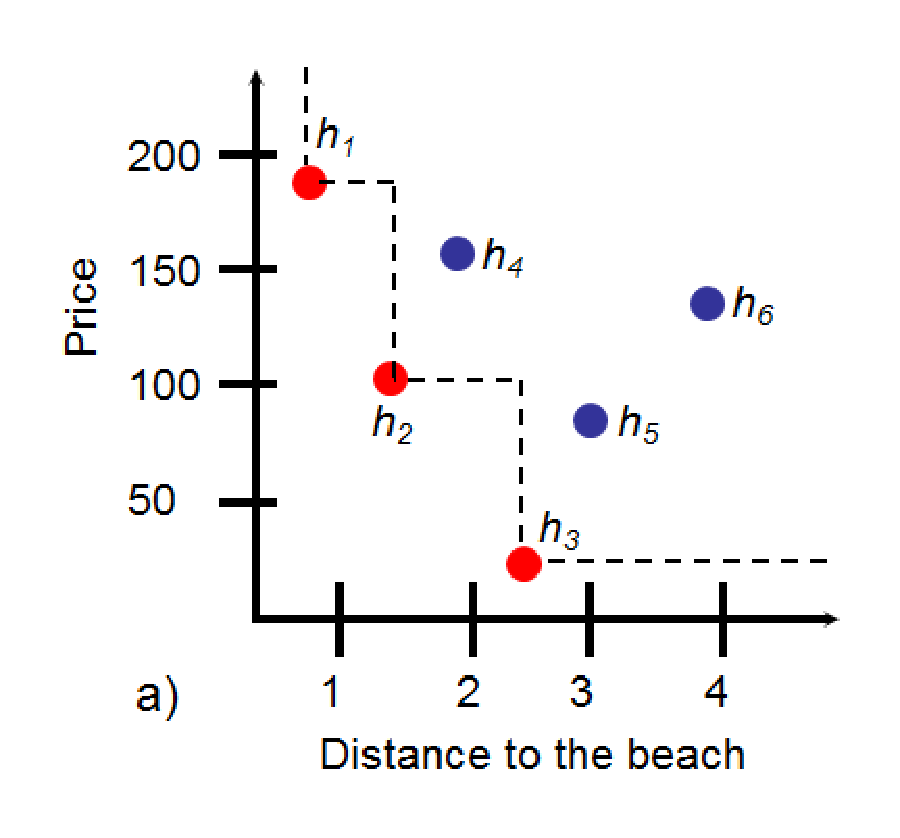
\includegraphics[width=5.5cm]{img/TraditSkyline.eps}
\caption{Skyline of a hotel search scenario}
\label{fig:TraditSkyline}
\end{center}
\end{figure}

Skyline queries were first studied as maximal vectors \cite{KLP75}. B\"orzs\"onyi et al. \cite{BKS01}, that introduced skyline queries for database applications, presented divide-and-conquer techniques and index structures to solve the problem in $O(n \log^{d-2} n + n \log n)$ time. Since then, a number of different sequential  \cite{KRR02, PTFS05,GSG07} and parallel \cite{CLY12, PMS13, MPLZ14} algorithms for the basic skyline computation have been proposed. In \cite{WZSK17} there is a good summary of them.

For completeness, we want to mention that the basic skyline problem has some generalizations.  For instances, there exist studies dealing with dynamic skylines queries, where there is a moving point of interest, this makes that the distance from this point to the candidates changes \cite{PTFS05, SS06, TXP07, LPYL11}. Some other papers discuss the reverse skyline queries which study the changes in the set of skylines when a new candidate is added. The solutions to this last problem are based on the dynamic problem \cite{DS07, GLZ14}. There also exist skylines queries in temporary databases, where the period of validity or existence of the candidates changes throughout the year, for example simulating hotels opening only in summer \cite{KTM17}. To end with, in \cite{GLCCL15} it is proposed the most desirable skyline object query, which returns the top dominating objects based on a ranking criterion that considers the number of objects dominated by a skyline object and their accumulated weights.


\vspace{1em}
{\it Spatial Skylines with Euclidean distance}.
Given a set $P$ of $n$ data points and a set $Q$ of $m$ query points in the plane, the {\it nearest spatial skyline query} (NSSQ) retrieves the points of $P$ such that no other point of $P$ is closer to all of the query points of $Q$ simultaneously. Let us see an example. A visitor of a trade fair identifies a set of city locations, say for example the central train station $c$ and the exhibition center venue $v$, and wants to select interesting hotels in terms of Euclidean distance. \iffalse Accordingly, $Q = \{c,v\}$ and $P$ contains the hotels, \fi
Considering the scenery depicted in Figure \ref{fig:SDExample1}, we want to select the hotels that are no father simultaneously from $c$ and $v$ than any other hotel. Thus,the spatial skyline hotels $h_1$, $h_2$ and $h_4$ with respect to $c$ and $v$ are the most interesting hotels for the visitor.
%Considering the scenery depicted in Figure \ref{fig:NSSQExample1}, we want to select the hotels that are no father simultaneously from $q_1$ and $q_2$ than any other hotel. Thus,the spatial skyline hotels $p_1$, $p_2$ and $p_4$ with respect to $q_1$ and $q_2$ are the most interesting hotels for the visitor.
This problem is a two-dimensional problem, because for each hotel two properties are analyzed. The analyzed elements can be turned into real data and each candidate can be mapped into a point in $\mathbb{R}^2$ with coordinates equal to the distance to the beach and its price. Thus, can be transformed to a traditional skyline problem of dimension 2.



        \begin{figure}[!htp]
        \begin{center}
        %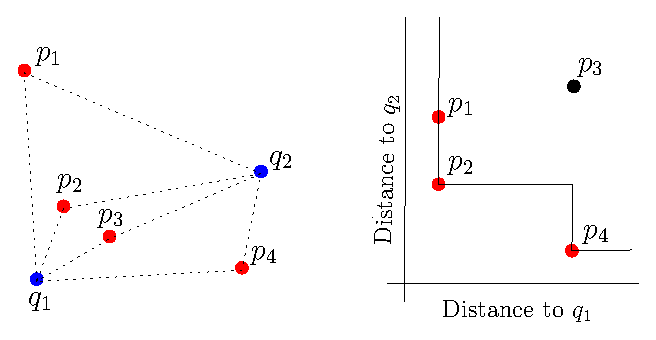
\includegraphics[width=0.5\linewidth]{img/SSQExample0_nou.eps}
        %\caption{Nearest spatial skyline hotels: $p_1$, $p_2$ and $p_4$.}
        %\caption{Point $p_2$ is a nearest spatial skyline and spatially dominates from near $p_1$. Between $p_1$ and $p_4$ no spatially dominance from near relation exists. }

        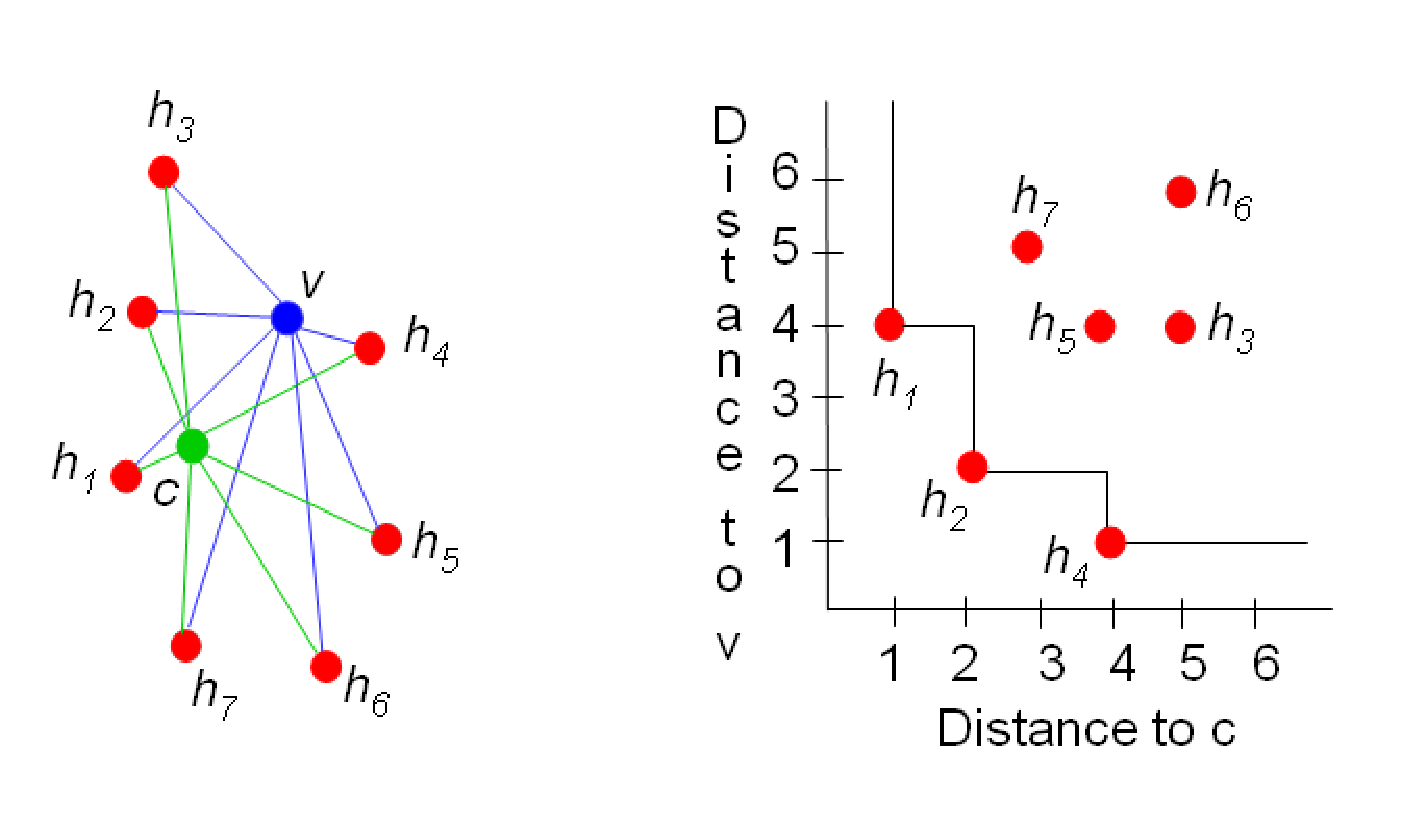
\includegraphics[width=9cm]{img/SSQExample1.eps}
        \caption{Nearest spatial skyline hotels: $h_1$, $h_2$ and $h_4$}
        \label{fig:SDExample1}
        \end{center}
        \end{figure}


 There can be applications of this problem in other areas, such as: events organization, disaster management decisions or facility location, among others. For instance, suppose that the members of a multidisciplinary task team that work in different offices, need to meet together regularly. The set of query points corresponds to the locations of the offices where the members usually work and the set of points of interest to the potential locations for their weekly meetings. Then, the best location for their weekly meeting is one of the skyline points. In disaster management, suppose that several residential buildings, defining the set of points of interest, must be evacuated because of several explosions or fires defining the query points. The first buildings to be evacuated are the spatial skylines buildings. Finally, consider a business plan for opening a number of shops, points of interest, near a set of residential areas, that define the set of query points. Again, the best locations for opening the new shops are the spatial skyline locations. Crisis management applications is another example: assume that a number of waterborne infectious disease cases were confirmed at different locations. People who live at spatial skyline places with respect to those locations should be alerted and examined first, because there might be a higher possibility that these people may have been exposed to contagious water.

 \vspace{1em}
 Analogously, given a set $P$ of $n$ data points and a set $Q$ of $m$ query points in the plane, the {\it farthest spatial skyline query} (FSSQ) retrieves the points of $P$ such that no other point of $P$ is farther from all of the query points of $Q$ simultaneously. Such queries are helpful in identifying spatial locations faraway from undesirable locations, e.g., unpleasant facilities (nuclear power plants, garbage dumps or chemical plants) or business competitors (hotels, restaurants). Figure \ref{fig:FSSQExample1} illustrates an example where we aim at finding an optimal subset of locations among 10 potential locations for a new park. We want the park to be far, in terms of Euclidean distance, from two query points that represent a chemical plant and a garbage dump. The most desirable locations for the park are the farthest spatial skyline locations $p_3$, $p_6$ and $p_7$.

 \begin{figure}[!htp]
 \begin{center}
 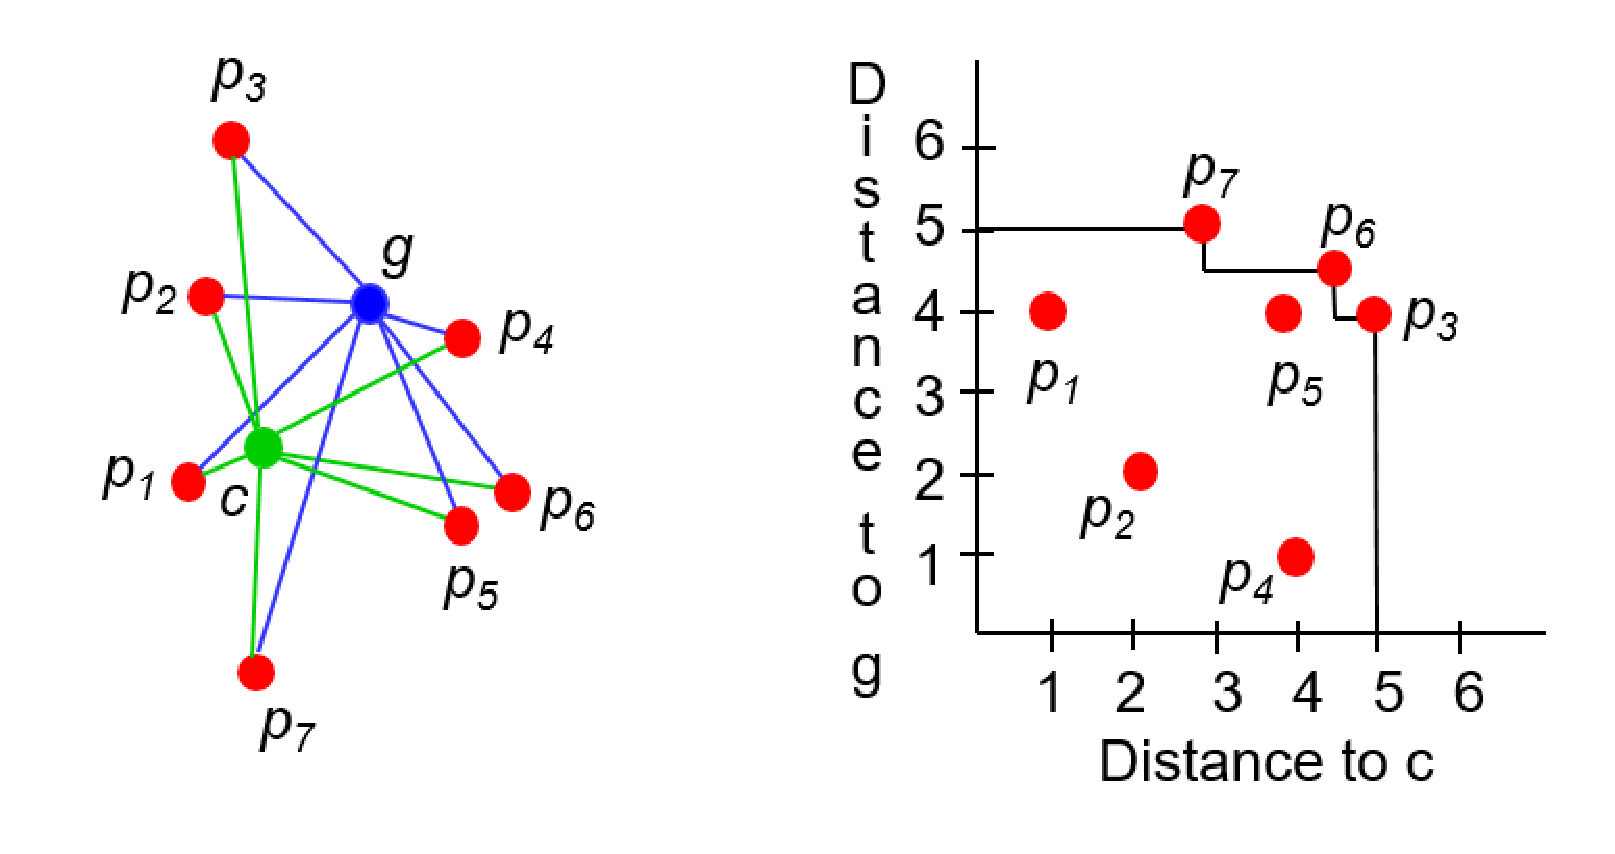
\includegraphics[width=9cm]{img/FarthestSkylineExample.eps}
 \caption{Farthest spatial skyline parks: $p_3$, $p_6$ and $p_7$}
 \label{fig:FSSQExample1}
 \end{center}
 \end{figure}


\vspace{1em}
Any NSSQ or FSSQ problem can be treated as a basic $d$-dimensional skyline query, considering for each point of interest its distance to each query point.
Applying the method of B\"orzs\"onyi et al. \cite{BKS01} nearest and farthest spatial skyline queries can be solved in $O(n \log^{m-2} n + n \log n)$ time if all the $O(nm)$ distances are already computed. Note that distances need to be recomputed for each different data set query $Q$. The goal of existent approaches is to efficiently solve spatial skyline queries, exploiting the
geometric properties of the problem, without such transformation \cite{SS06, SSK09, BBCDKS10, LSAH11, SB13,LZZ13}. Sharifzadeh and Shahabi \cite{SS06,SSK09} first introduced spatial skyline queries and presented R-tree based and Voronoi-based algorithms for solving the problem. By exploiting geometric properties, they avoid the exhaustive examination of all the point pairs in $P$ and $Q$. Bhattacharya et al. \cite{BBCDKS10}, reduce the spatial skyline problem to the problem of finding data points that have non-empty cells in an additively weighted Voronoi diagram under convex distance function. The weights of the Voronoi diagram are derived from the co-ordinates of the points of $P$ and the convex distance function is derived from $Q$. They present a \iffalse $O((n + m) \log m + n \log n)$-time \fi randomized incremental algorithm to find the set of non-dominated points. No results of the algorithm implementation are reported. Lee et al. \cite{LSAH11} take advantage of some geometric properties to sort the candidate points from less to greater distance to a query point to speedup the answers. \iffalse The time complexity of the algorithm is $O(n |S| \log |CH(Q)| + n \log n)$, where $S$ denotes the set of non-dominated points and $CH(Q)$ the convex hull of $Q$, that in the worst case is $O(n^2 \log m + n \log n)$. \fi This is, by now, the best existing sequential algorithm to solve the NSSQ problem. The same paper also provides an approximate algorithm to select a representative subset of skylines at a much lower cost. They also analyze the problem when considering a dynamic set of query points. Finally, Wenly et al. \cite{WZSK17} provide the only existent parallel solution for the NSSQ problem that uses the MapReduce technique.

The furthest spatial skyline query FSSQ problem has been studied in \cite{YLIH13}. First the problem is solved with a baseline algorithm and, then, an efficient progressive algorithm is proposed. The latter significantly outperforms the former by exploiting spatial locality. They also develop an efficient approximation algorithm to trade accuracy for efficiency.

\vspace{1em}
{\it General spatial skylines}. General spatial skyline query (GSSQ) was introduced at the same time by Lin et al. under this name \cite{LZZ13} and by Soudani and Baraani-Dastgerdi under the name of the spatial nearest neighbor skyline query \cite{SB13}. Instead of a single set of query points, they considered several sets of query points $Q_1$, $Q_2$, ..., $Q_l$ of different types. In this case, it is wanted to select, for example, the set of desirable {\it hotels} among a set of candidates such that there is no other hotel that has a beach, a shopping center, a public transport stop and a museum closer. Therefore, the query or candidate points are analyzed in relation to the distance to the nearest point of each set of query points $Q_i$.

\vspace{1em}
{\it Spatial skyline queries with non-Euclidean distance}. There exist algorithms to obtain the skylines using road-network distances \cite{SSK09} and Manhattan distance \cite{SHA14}. They both face the same problem but analyzing proximity with a different distance function. In fact, the only difference is the way in which proximity is measured because both use a metric function that has exactly the same properties as the Euclidean distance.

\vspace{1em}
{\it Top-$k$ spatial skyline queries}. In this case, the subset of the top-$k$ spatial skylines is selected among all the existent spatial skylines. The top-$k$ spatial skylines are the $k$ skylines optimizing a specific objective function. There are several papers dealing with top-$k$ spatial skylines \cite{PS14, SSKA17}. Son et al. \cite{SSKA17} deal with top-$k$ spatial skylines under Manhattan and Eudlidean distances. Particularly, they improve an existent approach for the Manhattan distance and present a solution to obtain the top-$k$ skylines.\\

\subsection{Our contributions}

In this paper, we study, for the first time, {\it nearest and farthest weighted spatial skyline queries}, i.e. nearest and farthest spatial skyline queries considering multiplicative weighted Euclidean distances, and extract the top-$k$ ones, if desired.

We summarize the geometric properties used to solve the spatial skyline queries under the Euclidean distance and analyze them under the weighted Euclidean distance. In fact, we show how most of them are not valid when considering multiplicative weighted Euclidean distances, in many cases, because it is not a metric function.

Moreover, in working towards practical solutions, we solve the nearest and farthest spatial weighted skyline queries with a sequential algorithm, but also with a GPU-parallel algorithm, under CUDA architecture. We theoretically and experimentally analyze both approaches and show the efficiency, robustness and fast running times of the parallel one. We also present the interface we developed to deal with this problem.

\subsection{Organization of the paper}

After presenting, in this introductory section, the traditional skyline and spatial skyline problems, we organize the remainder of the paper as follows. In Section \ref{sec:Background}, we provide the background of the spatial skyline under the Euclidean distance, the properties and existent algorithms to solve the nearest, farthest and top-k version of the problem.  In Section~\ref{sec:Theoretical_study}, we study the properties of the spatial skyline problem under the weighted Euclidean distance and compare them with the Euclidean spatial skyline problem properties. In Section~\ref{sec:Algorithms}, we present the sequential and the parallel algorithm to solve the weighted spatial skyline problem and theoretically analyze and compare them. The changes in the algorithms to efficiently extract the top-$k$ ones are presented in Section~\ref{sec:top_k}. Section~\ref{sec:ExpResults} contains the experimental results. Here, we present the developed interface to work with the weighted spatial skyline problem, experimentally analyze and compare the presented algorithms to solve the problem and sketch several alternative algorithms to solve the problem that have been analyzed and discarded according to their running times. Finally, conclusions are presented in Section~\ref{sec:Conclusions}.

\section{Background} \label{sec:Background}

In this Section, we provide the background for the spatial skyline queries. We start with the formal definition of the problem, the most important and used properties of the unweighted spatial skyline queries and the existent algorithms designed to solve them. Several of these properties and most of the algorithms relay on geometric aspects that are not true when a not metric function is used to measure proximity, which is the case of the multiplicative weighted Euclidean distance. %We do not extensively provide all the existent properties but only those that are meaningful for the new results we present in this paper.
We start with the more studied problem, the nearest spatial skyline queries, continue with the farthest spatial skyline problem and end with the nearest and farthest top-$k$ spatial skyline queries.

\vspace{1em}
We denote by $P$ a set of $n$ points of interest and by $Q$ a set of $m$ query points in the Euclidean plane. The Euclidean distance between points $p$ and $q$ is denoted $d(p,q)$.

\subsection{Nearest spatial skyline queries}

When referring to the nearest spatial skyline queries (under the Eudlidean distance), it is said that:

\vspace{0.6em}
 \begin{itemize}
  \item {\it $p_i$ spatially dominates from near $p_j$} $\iff$ $d(p_i, q_k) \le d(p_j, q_k) \; \forall q_k\in Q$ and $\exists q_l\in Q \ d(p_i, q_l) < d(p_j, q_l)$ \vspace{0.6em}% (see Figure \ref{fig:SDExample1})\\
  \item {\it $p_i$ is not spatially dominated from near by $p_j$} $\iff$ $\exists q_k\in Q$ with $d(p_i, q_k) < d(p_j, q_k)$
            \begin{flushright}
                 {or $d(p_i, q_k) = d(p_j, q_k) \forall q_k \in Q$ \hspace{0.2\linewidth }\vspace{0.6em}}
                   \end{flushright}% (see Figure \ref{fig:SDExample1})\\
  \item {\it $p_i$ is a nearest spatial skyline point} $\iff$ $p_i$ is not spatially dominated from near by any other point of $P$\vspace{0.6em}
 \end{itemize}

 According to the previous definitions, the terms {\it nearest spatial skyline points} and {\it non spatially dominated points from near } can be interchangeably used. In the example of Figure~\ref{fig:SDExample1}, point $h_2$ spatially dominates from near $h_5$ but it is not spatially dominated from near by any other point of $P$. Hence $h_2$ is a spatial nearest skyline point. The same happens with $h_1$ and $h_4$.\\

        In fact, the {\it nearest spatial skyline query} is formally defined as the problem of retrieving the set $NSSQ(P,Q)$ of all the nearest spatial skyline points of the set $P$  with respect to $Q$, or equivalently all the points that are not spatially dominated from near by any point in $P$. In Figure~\ref{fig:SDExample1}, the nearest spatial skyline query would report the set $NSSQ(P,Q) = \{p_1, p_2, p_4\}$.\\

        The nearest spatial skyline points can be easily obtained by checking, for each point in $P$, whether it is spatially dominated from near by any other point in $P$ with respect to $Q$. However, there exist several geometric properties of the set of nearest spatial skyline points that restrict the region where the nearest spatial skyline point can be located. These properties can be used to design more efficient algorithms avoiding some dominance tests. Next, we summarize the most important definitions and lemmas of the nearest spatial skyline points. \\
        \begin{itemize}
        \item {\it Closest region to $p_i$ with respect to $p_j$}: $r(p_i,p_j)$ is the set of points of the Euclidean plane closer to $p_i$ than to $p_j$, it is the half plane containing $p_i$ and delimited by the bisector $b(p_i, p_j)$ of the points $p_i$ and $p_j$. The bisector $b(p_i,p_j)$ is the locus of equidistant points between $p_i$ and $p_j$ that defines the straight line perpendicular to the line connecting $p_i$ and $p_j$ through their midpoint. \vspace{0.6em}

        \item {\it Convex hull of $Q$}: $CH(Q)$ denotes the {\it convex hull} or {\it convex envelope} of the set of points $Q$ which is the smallest convex set that contains $Q$. Its vertices are called {\it extreme points} and define the set $E(Q)$.\vspace{0.6em}

        \item {\it Voronoi diagram of $P$}: $VD(P)$ denotes the {\it Voronoi diagram} of $P$ defined by the planar partition of the Euclidean plain in to $|P|$ cells, one associated to each point $p_i\in P$, called the Voronoi cell of $p_i$ which contains the points of plane that are closer to $p_i$ than to any other point in $P\setminus \{p_i\}$. \vspace{0.6em}

        \item {\it Independent region of $p$ and $q$}: $D(q,p)$ is the disk centered at $q$ and radius $d(q,p)$ \cite{WZSK17}. \vspace{0.6em}

        \item {\it Search region} also called {\it Independent Region Group} of $p_i$ with respect to $Q$: $SR(p_i,Q)$ includes $p_i$ and all the points of $P$ that are not spatially dominated by $p_i$, and hence the spatial skyline is contained in $SR(p_i,Q)$  $\forall p_i\in P$. It is defined as $$SR(p_i,Q) = \bigcup_{q_k \in Q} D(q_k, p_i).$$

        \item {\it Dominator region} of $p_i$ with respect to $Q$: denotes  the region that is dominated by $p_i$, it is defined as
            $$DR(p_i,Q)=\bigcap_{q_k \in Q} D(q_k, p_i) \, .$$\vspace{0.6em}
        \end{itemize}


\iffalse        In the three charts of Figure~\ref{fig:NDR1i2} we depict a set $Q=\{q_1, q_2\}$ and several sets $P$ corresponding to several spatial skyline problems in different charts. The disks involved in the search and in the dominator regions of a point $p_i$ are the two disks colored in the same color and that go through $p_i$. Their union define the search region of $p_i$ and their intersection the dominator region of $p_i$ with respect to $Q$.
        \begin{figure}[!htp]
            \begin{center}
            
\includegraphics[width=0.9\linewidth]{img/search_regions.eps}
            %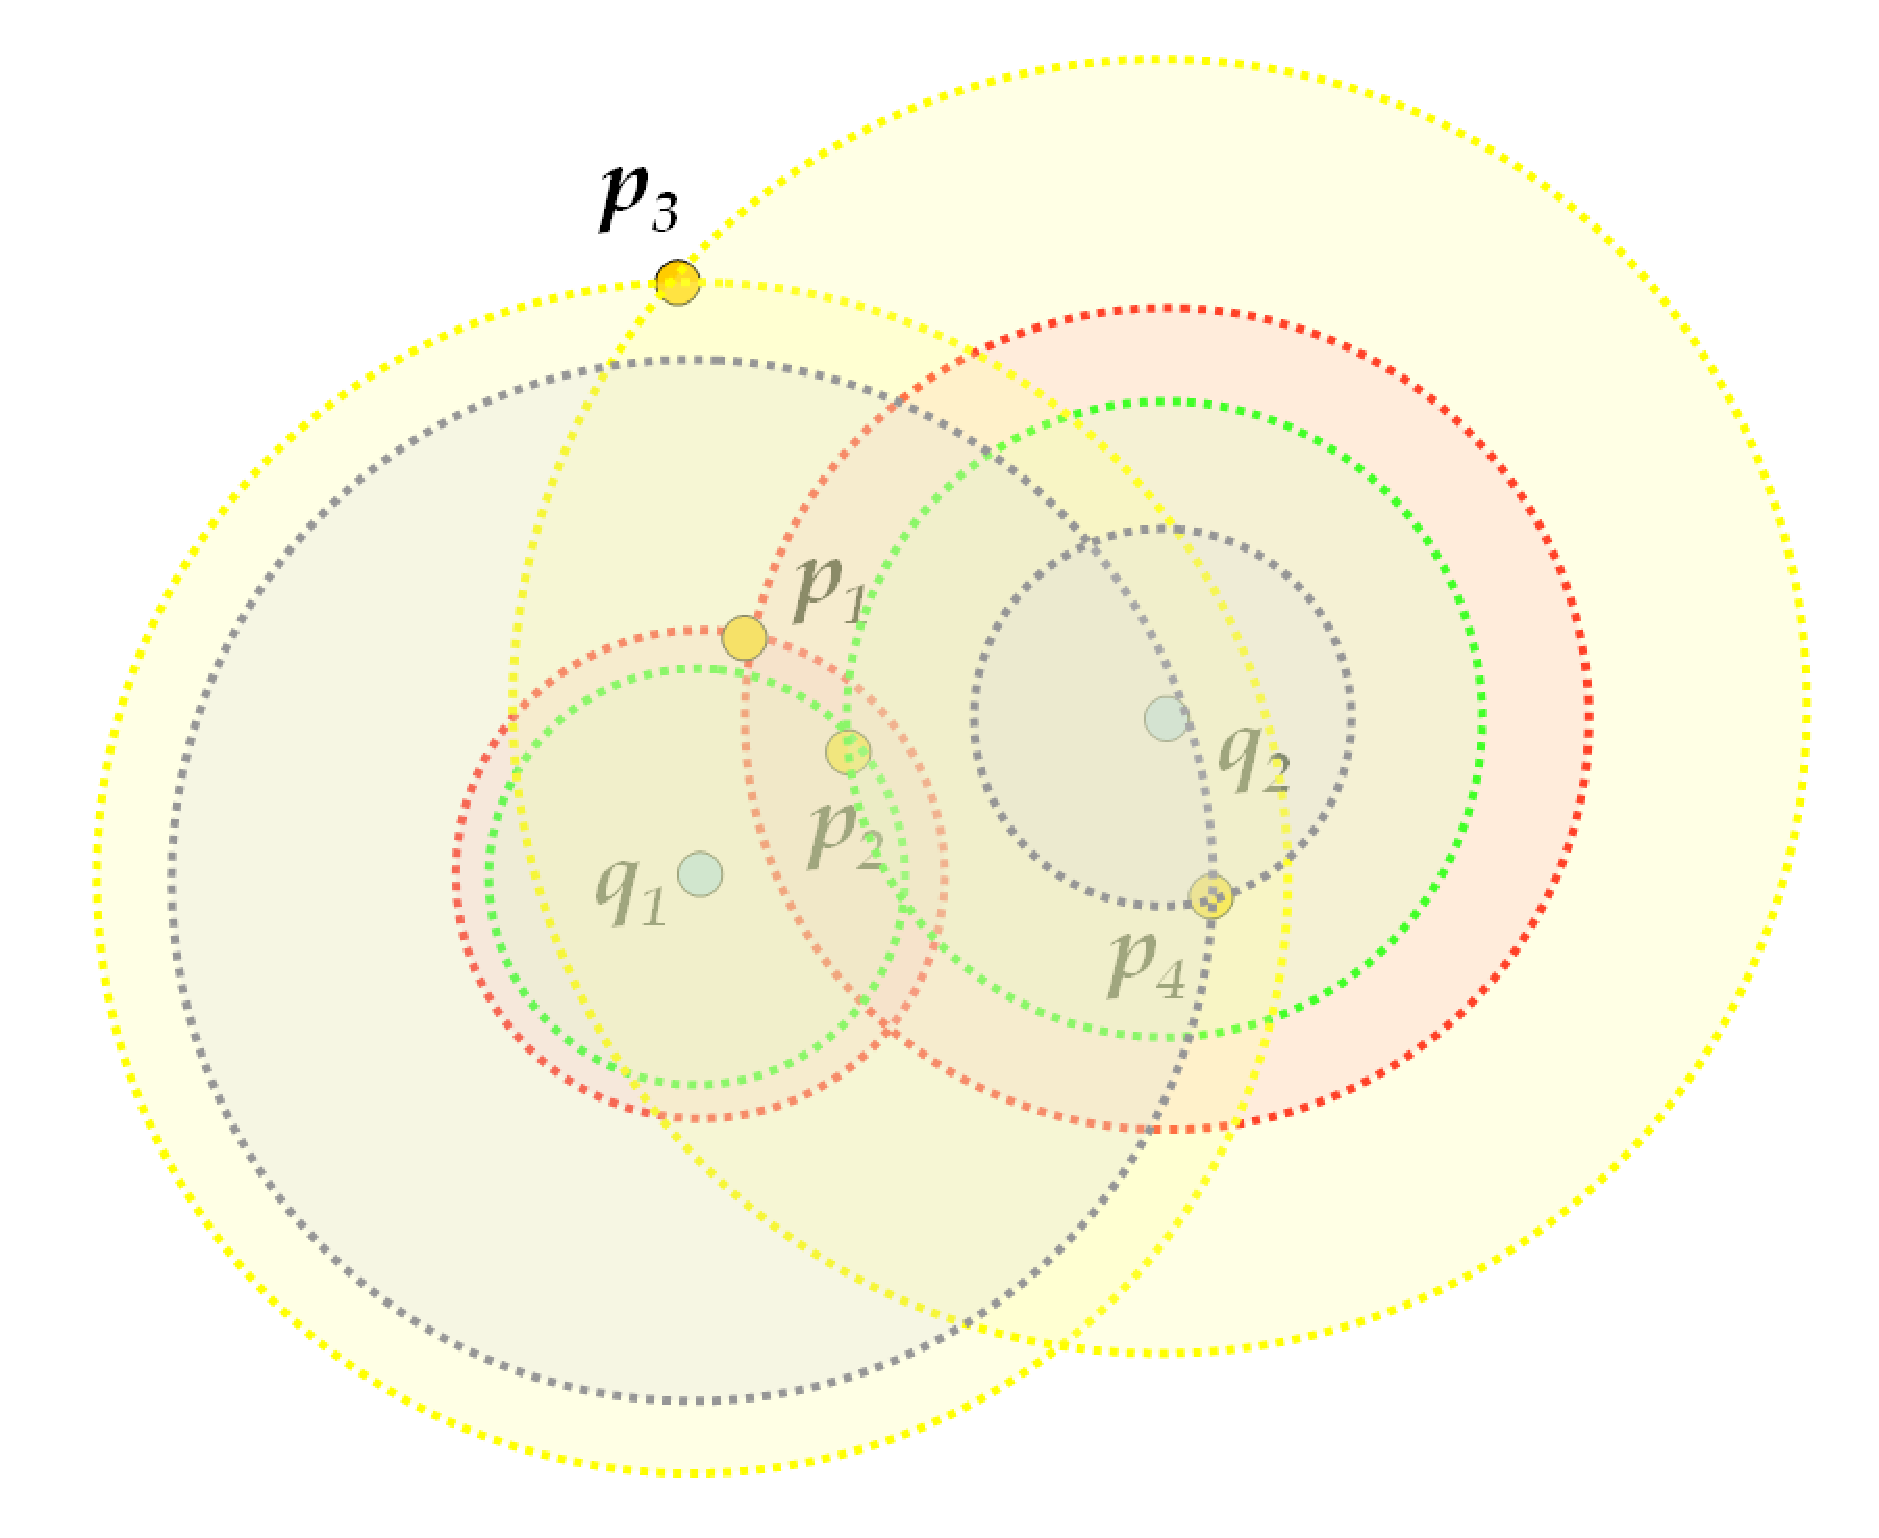
\includegraphics[width=4.76cm]{img/RegNonDominance3.eps} \hspace{-1.5em} a)
            %\includegraphics[width=5.75cm]{img/RegNonDominance1.eps} \hspace{-1.5em} b)
            %\includegraphics[width=5.75cm]{img/RegNonDominance2.eps} \hspace{-1.5em} c)
            \caption{a) $SSQ(P,Q) = \{p_2,p_4 \}$, b) $SSQ(P,Q) = \{p_1,p_2
            \}$, c) $SSQ(P,Q) = \{p_1 \}$} \label{fig:NDR1i2}
            \end{center}
        \end{figure} \fi

        The search and dominator regions restrict the region where the skyline points can be located to a bounded region of the Euclidean plane and provide a characterization of the skyline points. This is stated in the following lemmas.\\

        \begin{lemma}
            The spatial skyline is contained in the intersection of all the search regions which is, meanwhile, contained in the intersection of the search regions of the points of any subset $P'\subset P$, i.e.  %$P' \subset P$, $$SSQ(P,Q) \subset \bigcap_{p_i \in P} SR(p_i,Q) \subset \bigcap_{p_i \in P'} SR(p_i,Q)\ .$$
             $$NSSQ(P,Q) \subset \bigcap_{p_i\in P} SR(p_i,Q) \subset \bigcap_{p_i \in P'} SR(p_i,Q)\ \text{ for any } P' \subset P.$$
            \label{lemma:SearchRegion}
        \end{lemma}

        \begin{lemma} A point $p_i$ is a skyline point if and only if it is the only point of $P$ contained in its dominator region $DR(p_i,Q)$, i.e. $$ p_i \text{ is a skyline point } \iff P \cap DR(p_i,Q)= \{p_i \}.$$ %Consequently  $SSQ(P,Q) = \{ p_i \in P \, | \, P \cap DR(p_i,Q)  = \{p_i \} \}$.
        \label{lemma:SkylinePoints2}
        \end{lemma}

        According to Lemma~\ref{lemma:SkylinePoints2} the spatial skyline can be obtained as the set of points of $P$ whose dominator region does not contain any other point of $P$, i.e. $$ NSSQ(P,Q) = \{ p_i \in P \, | \, P \cap DR(p_i,Q)  = \{p_i \} \}.\vspace{0.6em}$$



         %In this Section we rewrite some lemmas borrowed from \cite{SSK09} and \cite{LSAH11}. In fact, Lemma \ref{lemma:IntBisectorCH} reduces the test of spatial dominance between two points to check whether their bisector intersects $CH(Q)$. Lemma \ref{lemma:ExtremePoints} allows us to compute $SSQ(P,Q)$ as
        %        $SSQ(P,E(Q))$ reducing the set $Q$ to the set extreme points, $E(Q)$. Lemma \ref{lemma:SkylinePoints} provides a subset of
        %        skyline points by determining those points of $P$ contained inside $CH(E(Q))$. Finally, Lemma \ref{lemma:ClosestPoints}, together with Lemma
        %        \ref{lemma:ExtremePoints},  proves that the points of $P$ that are closer to a point of $E(Q)$ are also skyline points. \todecide{Aquest ultim crec q no es fa servir!}\\

        There also exist several other important properties that help in the detection of the spatial skyline and that are used in the algorithms proposed to solve the problem.\vspace{0.6em}

        %\begin{lemma} Being $q\in Q$ and $p_i\in P$, $D(q,p_i)$ is an {\it independent region}, because any point $p\in D(q,p_i) \cap P$ can only be dominated by a point of $P \cap D(q,p_i)$.

        \begin{lemma} Being $q\in Q$ and $p_i\in P$, any point $p\in D(q,p_i) \cap P$ can only be dominated by a point of $P \cap D(q,p_i)$.
        \label{lemma:indep_regions} \end{lemma} \vspace{0.6cm}

        \begin{lemma} If $E(Q) \subset r(p_i, p_j)$ then $p_i$ spatially dominates $p_j$.  \label{lemma:FIntHalfSpaceCH} \end{lemma} \vspace{0.6em}

        \begin{lemma} The bisector of two data points in $P$ intersects the interior of $CH(Q)$ if and only if they do not spatially dominate each other. \label{lemma:bisector}\end{lemma} \vspace{0.6em}

        \begin{lemma} The set of skyline points of $P$ with respect to $Q$ depends only on $E(Q)$, which defines $CH(Q)$. \label{lemma:useExtremePoints}\end{lemma}\vspace{0.6em}

        \begin{lemma} Each point $p \in P$ that is inside $CH(Q)$ is a skyline point. \label{lemma:inCH_SK}\end{lemma}\vspace{0.6em}

        \begin{lemma} The closest point $p_j \in P$  to point $q_k \in Q$, assuming uniqueness, is a spatial skyline point. \label{lemma:clossest_point}\end{lemma}\vspace{0.6em}

        \begin{lemma} Each $p\in P$ whose Voronoi cell intersects the interior of $CH(Q)$ is a spatial skyline point. \label{lemma:VCell}\end{lemma}\vspace{0.6em}

        \begin{lemma} If point $p_i\in P$ spatially dominates $p_j\in P$ and $p_j$ spatially dominates $p_k\in P$, then $p_i$ spatially dominates $p_k$. \label{lemma:transitive} \end{lemma}\vspace{0.6em}

        %\begin{enumerate}
        %        \item The bisector of two data points in $P$ intersects the interior of $CH(Q)$ if and only if they do not spatially dominate each other.
        %        \item The set of skyline points of $P$ with respect to $Q$ depends only on the points defining $CH(Q)$, which are called extreme points of $Q$ and its set is denoted by $E(Q)$.
        %        \item Each point $p \in P$ that is inside $CH(Q)$ is a skyline point.
        %        \item The closest point $p_j \in P$  to point $q_k \in Q$, assuming uniqueness, is a spatial skyline point.
        %    \end{enumerate}


\subsubsection{Existent algorithms}

There exist several approximated and exact algorithms to solve nearest spatial skyline queries. Among them, we briefly explain the most relevant and used ones. We do not pay attention to the approximated ones because are not directly related to our work. We explain the force brute algorithm to solve the problem, the fastest sequential one and the most known algorithm used until the fastest one was presented. Finally, we also present the fastest parallel algorithm.\\

%      Force brute algorithm

 The simplest algorithm, the {\it brute force algorithm} ($BF$), analyzes all the pairs $(p_i, p_j) \in  P \times P$ with $i\neq j$ and performs its dominance test, i.e. it checks whether $p_j$ dominates $p_i$. If $p_i$ is not dominated by any point $p_j\in P-\{p_i\}$ the point $p_i$ is set as a spatial skyline. The dominance test associated to $p_i$ and $p_j$ can be done considering the half-space of $p_i$ with respect to $p_j$,  $h(p_i, p_j)$. Since $p_j$ dominates $p_i$ if all the points of $Q$ are closer to $p_j$ than to $p_i$; it is checked whether there exists a point $q_k \in Q$ lying in $h(p_i, p_j)$. If such a point exists for every $q_j$, $p_i$ is stored as a skyline point. Checking wether a point $p_i\in P$ is a spatial skyline point with this algorithm takes $O(nm)$ time in the worst case. Hence, the total time complexity of this force brute algorithm $O(n^2m)$. This algorithm can be easily improved by considering $E(Q)$ instead of $Q$ (Lemma~\ref{lemma:useExtremePoints}), this reduces the worst case time complexity to $O(n^2 m')$, where $m'=|E(Q)|$. Moreover, the dominance test can be also accelerated by using Lemma~\ref{lemma:bisector} and an appropriate algorithm to check whether the bisector of the two points intersects the convex polygon $CH(Q)$, the time complexity of these {\it accelerated brute force} algorithm ($ABF$) is reduced to $O(n^2 \log m')$.\\

%      Fastest existent exact algorithm

        %Sharifzadeh et al. \cite{SSK09} presented an algorithm to obtain the skyline that uses most of the presented properties. In fact they provided two years before a first algorithm \cite{SS06} that contained several errors that themselves posteriorly fixed. In fact \cite{ssk09} is where the unique parallel algorithm to solve the problem relies. They start determining $CH(Q)$ to reduce $Q$ to $E(Q)$ (Lemma~\ref{lemma:useExtremePoints}) and compute $VD(P)$. Then, they set the points of $P$ contained in $CH(Q)$ to the set of skyline points (Lemma~\ref{lemma:inCH_SK}), the same is done with those points of $P$ whose Voronoi diagram cell intersects the interior of $CH(Q)$ (Lemma~\ref{lemma:VCell}). Since all the interior points have already been added they only have to intersect $VD(P)$ with $CH(Q)$ which can be easily and smartly done with an appropriate algorithm that determine the intersections of the planar subdivisions. Then, they select a set $C$ of candidates to skyline points by using the search regions (Lemma~\ref{lemma:SearchRegion}). In fact, the search region is roughly approximated by its bounding box to make the computation easier. The set of potential skylines $C$ contains the points in $P-SS$ contained in the bounding box defined as the intersection of all bounding boxes containing the search regions of the already found skyline points. The set $C$ is obtained by using a R*-tree, then the points of $C$ are sorted in ascending order of the distance between the candidates and a point $q\in E(Q)$. They check whether each candidates is dominated by one of the already found skylines, checking whether their bisector intersects the boundary of $CH(Q)$ (Lemma~\ref{lemma:bisector}). If the point is the only point in the search region it is obviously set as a spatial skyline point (Lemma~\ref{lemma:SkylinePoints2}). When a new skyline if found the bounding box is updated so that it keeps on being the intersection of all the bounding boxes of all the search regions of the already detected skylines. Thus, if when they check a new candidate it is not contained in the updated bounding box it is directly discarded as avoiding the dominance test. They prove that the worst case complexity of this algorithm is $O(n(s\log m' +\log n) + m\log m)$, where $s=|S|$, in fact, since usually $m\le n$ the complexity is in $O(n(s\log m'+\log n))$. Note that in the worst case $s=O(n)$ and it becomes again $O(n^2\log m')$. But the running times of this algorithm are usually much smaller than those obtained with the brute force algorithm.

        Sharifzadeh et al  \cite{SS06} proposed the Banch-and-bond spatial skyline algorithm ($B^2S^2$) that searches the spatial skyline candidates by visiting an R-tree from top to bottom which avoids several dominance tests. They also presented the Voroni-based Spatial Skyline ($VS^2$) which starts with the closest data points to query points and searches in the space by visiting the neighbors of the visited data points over the Voronoi diagram. They used Lemmas~\ref{lemma:SearchRegion},~\ref{lemma:SkylinePoints2},~\ref{lemma:useExtremePoints},~\ref{lemma:inCH_SK}, and~\ref{lemma:clossest_point}. In their experiments $VS^2$ preformed better than $B^2S^2$. However, themselves posteriorly show that the version of the $VS^2$ that had proposed was not completely correct and fixed the errors in~\cite{SSK09} by using Lemma~\ref{lemma:VCell}. Fixing the errors lowered the performance of the algorithm, but it was still the best algorithm at that moment.\\

        Posteriorly, Lee et al. presented the fastest known algorithm in \cite{LSAH11}, which we call {\it distance-sorting} ($DS$). They manage to notoriously reduce the number of tests done. After reducing $Q$ to $E(Q)$ (Lemma~\ref{lemma:useExtremePoints}) they select an arbitrary point $q\in E(Q)$ and sort the points of $P$ according to increasing distance to $q$. Then, they start finding the spatial skyline points; the closest point to $q$ is a spatial skyline point (Lemma~\ref{lemma:clossest_point}) and the rest of points of $P$ are analyzed in increasing distance to $q$ order. They use the transitivity of the dominance property and the fact that the point being analyzed can only be spatially dominated by the already detected skyline points (Lemma~\ref{lemma:transitive}). It drastically reduces, in practice, the number of performed dominance test. Again to check whether a point is dominated by any of the already obtained skylines, they check whether the bisector of the two points intersects the $CH(Q)$ (Lemma~\ref{lemma:bisector}). This algorithm takes $O(m\log m)$ to construct the convex hull, $O(n\log n)$ to sort $P$ in increasing distance order, and preforms $O(|S|)$ dominance tests in $O(\log m')$ time each, where $S$ denotes the set of non-dominated points. Since generally $m<n$ it leads to a total time complexity of $O(n(|S|m+\log n)$. Lee et al.~\cite{LSAH11} also provide a fastest approximate algorithm to solve the problem that consists in computing the $VD(P)$ and $CH(Q)$ and approximate the skyline by the set of spatial skyline points as the points of $P$ whose Voronoi cell intersects the interior of $CH(Q)$ which is a subset of the real skyline.\\

%        Existent parallel algorithm

     The first {\it parallel approach} ($PA$) to detect the spatial skyline was presented in \cite{WZSK17}. The approach relays on Lemma~\ref{lemma:useExtremePoints},~\ref{lemma:indep_regions} and~\ref{lemma:SearchRegion}. The base idea is that, each search region is the union of several disks that define an independent region when looking for spatial skyline points (Lemma~\ref{lemma:indep_regions}). Hence, they chose the search region defined by a point $p\in P$ which is called the {\it independent region pivot} and manage to turn the problem into $m'$ independent problems, one for each of the disks defining the search region. These $m'$ problems are solved in parallel. In fact, they propose a three-phase MapReduce-based solution. In the first phase they calculate $CH(Q)$, $Q$ is partitioned, several local convex hulls are first output and then merged to produce the global convex hull. In the second MapReduce-phase they determine the independent region pivot, they look for the point $p\in P$ whose search region has minimal area; the area of the search regions is first locally and then globally minimized. Finally, in the third phase each point of $P$ is associated to the independent regions defining the search region of the chosen pivot, where it is contained. Then $|E(Q)|$ independent spatial skyline problems are solved in parallel by using the independent regions and only the points contained in the independent region. They also avoid dominance tests by taking advantage of the pruning regions, which are defined by circular ring sectors, because the points inside these regions are dominated. The algorithm also uses two multi-level grids and ends by eliminating potentially repeated skyline points. This is necessary because the same skyline can be obtained in different independent regions and hence there will appear duplicated in the output.

       % \subsubsection{Fastest existent parallel algorithm}\label{alg:fastestCPU}

\subsection{Farthest spatial skyline queries}

The farthest spatial skyline query problem was first introduced in 2013 by You et al in \cite{YLIH13}. In that paper, they reverse proximity for remoteness. A point of interest $p\in P$ is desirable if no other point $p'\in P$ is farther from all the query points of $Q$. Unlike the nearest spatial skylines points that are clustered within around the query convex hull, the farthest ones are scattered across the entry data space. They prove that there does not exist duality between the nearest and farthest spatial skylines and provide the following problem definitions: \\

         \begin{itemize}
            \item {\it $p_i$ spatially dominates from far $p_j$} $\iff$ $d(p_i, q_k) \ge d(p_j, q_k) \; \forall q_k\in Q$ and $ \exists q_l\in Q \ d(p_i, q_l) > d(p_j, q_l)$ \vspace{0.6em}% (see Figure \ref{fig:SDExample1})\\
            \item {\it $p_i$ is not spatially dominated from far by $p_j$} $\iff$ $\exists q_k\in Q$ with $d(p_i, q_k) > d(p_j, q_k)$
            \begin{flushright}
                 {or $d(p_i, q_k) = d(p_j, q_k) \forall q_k \in Q$ \hspace{0.2\linewidth }\vspace{0.6em}}
                   \end{flushright}% (see Figure \ref{fig:SDExample1})\\
            \item {\it $p_i$ is a farthest spatial skyline point} $\iff$ $p_i$ is not spatially dominated from far by any other point of $P$\vspace{0.6em}
        \end{itemize}

         The {\it farthest spatial skyline query} is formally defined as the problem of retrieving the set $FSSQ(P,Q)$ of all the farthest spatial skyline points of the set $P$  with respect to $Q$, or equivalently of all the points that are not spatially dominated from far by any point in $P$. \\


        They prove how Lemma~\ref{lemma:bisector}, Lemma~\ref{lemma:useExtremePoints} and Lemma~\ref{lemma:transitive} also hold for the farthest spatial skyline points and provide the following properties.
        \vspace{1em}


        \begin{lemma} If $E(Q) \subset r(p_i, p_j)$ then $p_j$ spatially dominates from far $p_i$. \label{lemma:FIntHalfSpaceCH} \end{lemma} \vspace{0.6em}

        \begin{observation} A point of $P$ inside $CH(Q)$ may not be a farthest skyline point. \label{lemma:FInsideCH} \end{observation} \vspace{0.6em}

        \begin{lemma}  The farthest point $p_j \in P$  to point $q_k \in Q$, assuming uniqueness, is a farthest spatial skyline point. \label{lemma:clossest_point}\end{lemma}\vspace{0.6em}

        \begin{lemma} If the Voronoi region of a point of P intersects with $CH(Q)$ then the point does not dominate from far any other point of $P$. \label{lemma:FVoronoi} \end{lemma} \vspace{0.6em}

\subsubsection{Existent algorithms}

In \cite{YLIH13}, two solutions are proposed. One based on the transformation of the problem to a $n$-dimensional general skyline problem, in which the Improved Distributed Skyline (IDS) algorithm of \cite{BGZ04} is adapted by using an $R$-tree. The second proposal, the Branch-and-bound farthest spatial skyline ($BBFS$),  significantly outperforms the initial one by using the geometric properties of the problem. It uses Lemmas~\ref{lemma:inCH_SK}, Lemma~\ref{lemma:FVoronoi} and Lemma~\ref{lemma:transitive} indirectly, i.e., the fact that any point whose Voronoi diagram cell intersects $CH(Q)$ does not dominate from far any other point of $P$. In the paper, they also provide an approximate algorithm that reduces the processing cost without significantly affecting the quality of the results.
The paper does not provide the complexity of any of the two algorithms.


\subsection{Top-$k$ Nearest and Farthest Spatial Skyline Queries}

The top-$k$ spatial skyline query retrieves the subset of the best (lowest/highest scores) $k$ skyline objects with respect to $f$ for small $k$. With this aim, users specify some ranking function $f$ that reflects the relevance of each point in the skyline. A scoring function $f$ is said to be monotone if and only if for any two points $p$, $p'$, such that $d_p(q) \le d_{p'}(q)$ for every $q \in Q$, implies $f(p) \le f(p')$.
Typical monotone scoring functions are $$\delta_{max}(p) = \max_{q \in Q} d_p(q); \;\; \delta_{min}(p) = \min_{q \in Q} d_p(q)  \; \text{ and } \delta_{sum}(p) = \sum_{q \in Q} d_p(q).$$
The top-$k$ nearest spatial skyline points are the points minimizing the scoring functions and the furthest ones those maximizing them.\\

The existent studies on the top-$k$ skyline points deal with the nearest case, mobile environments \cite{PS14} and the Manhattan distance \cite{SSKA17}.

\section{Nearest and farthest weighted skyline queries}\label{sec:Theoretical_study}

In this section, we formalize the problem tackled in this paper which deals with the multiplicative weighted Euclidean distance and the nearest and farthest spatial skyline points. We start by defining the multiplicative weighted Euclidean distance and then analyze its properties and particularities, mainly in comparison with those of the Euclidean distance.

\subsection{Multiplicative weighted Euclidean distances}

Let $P$ be a set of points in the plane. Assume that each $p \in P$ is associated with a positive real weight $w_p > 0$. The {\it multiplicative weighted (Euclidean) distance} $d_p(q)$ from the location $p \in P$ to an arbitrary point $q$ is defined as $d_p(q)=(1/w_p)~d(p,q)$, where $d(p,q)$ denotes the {\it Euclidean distance} between points $p$ and $q$. Note that, the multiplicative weighted distances is a non-metric, it is not symmetric and the triangle inequality does not hold because the weights are point-depending.

\vspace{1em}
As an example, in Figure~\ref{fig:k-dissimilarity} we have a set $P$ of seven points and the squared query point $q$. In Figure~\ref{fig:k-dissimilarity}~a), where the Euclidean distance is considered, $q$ has one point at distance $u$, two points at distance $2u$, three points at distance $3u$ and one point at distance $4u$. In Figure~\ref{fig:k-dissimilarity}~b), where multiplicative weighted distances are considered, the weights of the points of $P$ are the ones represented in brackets. In this case, $P$ has two points at weighted distance $u$ from $q$, one point at weighted distance $2u$, two points at weighted distance $3u$ and two points at weighted distance $4u$. Note that, in Figure~\ref{fig:k-dissimilarity}~b) the point placed on the smallest semi-circumference has a weighted distance of $4u$ with respect to $q$, meanwhile the point placed on the greatest semi-circumference is only at weighted distance $2u$ from $q$.

        \begin{figure}[h]
        \begin{center}
        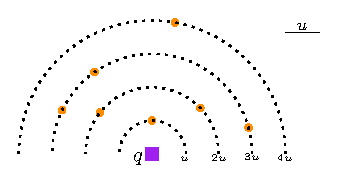
\includegraphics[width=0.4\linewidth]{img/knnExample.eps} \hspace{-0.5em} a) %k-dissimilarity.eps}
        \qquad
        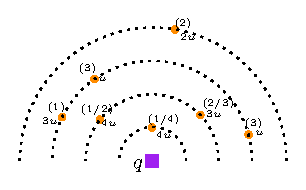
\includegraphics[width=0.4\linewidth]{img/knnExampleWeights.eps} \; b)
        \caption{a) Euclidean distances, b) multiplicative weighted Euclidean distances}
        \label{fig:k-dissimilarity}
        \end{center}
        \end{figure}\vspace{1em}


        %\subsection{Bisectors and nearest regions}
        %\vspace{1em}
        This multiplicative weight transforms the {\it shape} of several well known geometric elements used in the spatial skyline problems. Among others we remark the following ones. \\
        \begin{itemize}
        \item {\it Bisector between $p_i$ and $p_j$}, $b(i,j)$, becomes a circumference when $w_i\neq w_j$ and a line segment otherwise. According to the definition it is the locus of points at identical distance to $p_i$ and $p_j$, i.e. $$ b(i,j) = \{ s \in \mathbb{R}^2 \; | \; d_{p_i}(s)=d_{p_j}(s)\}  = \{ s \in \mathbb{R}^2 \; | \; d(p_i,s)/d(p_j,s)=w_{p_i}/w_{p_j}\}.$$ When $w_{p_i} / w_{p_j} \neq 1$ it defines the Apollonius circumference which has center $c_{ij}=(w_{p_i}^2 p_j - w_{p_j}^2 p_i)/(w_{p_i}^2 - w_{p_j}^2)$ and radius $r_{ij}=w_{p_i}w_{p_j} d(p_i,p_j)/|w_{p_i}^2 - w_{p_j}^2|$. The center $c_{ij}$ is aligned with $p_i$,  $p_j$ and does not separate them. On the contrary, when the weights are the same it defines a straight line.


        \begin{figure}[h]
        \begin{center}
        %\includegraphics[width=0.35\linewidth]{img/BisectorCircles.eps} a)
        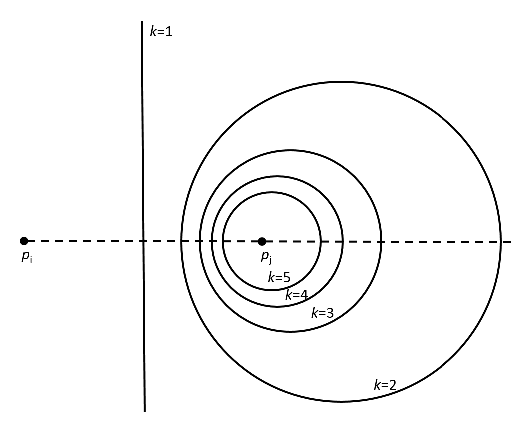
\includegraphics[width=0.35\linewidth]{img/bisectors_w.eps} a) \qquad
        
\includegraphics[width=0.3\linewidth]{img/vd_weighted.eps} b)
        \caption{a) Bisector circles for several ratios $k=w_{p_i}/w_{p_j}$, b) A Voronoi Diagram under weighted Euclidean distance }
        \label{fig:WD_Bis_VD}
        \end{center}
        \end{figure}


        Figure \ref{fig:WD_Bis_VD}~a) provides several examples of bisector circles $b(i,j)$ for fixed points $p_i$ and $p_j$ corresponding to different values of  $k=w_{p_i}/w_{p_j}$, where $k \ge 1$ is assumed without loss of generality. The circles always surround point $p_j$. As $k$ grows, the radius of the circles decreases and the center becomes closer to $p_j$. On the contrary, as $k$ diminish the radius of the circles increases and the center of the circles goes away from $p_j$. In the special case of $k = 1$ ($w_{p_i}=w_{p_j}$), the bisector becomes a straight line (circle of infinite radius).\vspace{0.6em}

        \item {\it Closest region to $p_i$ with respect to $p_j$}: $r(p_i,p_j)$ becomes to the planar region  bounded by $b(i,j)$ containing $p_i$, it may either by the interior or the exterior of the circle defined by $b(i,j)$. Regarding Figure~\ref{fig:WD_Bis_VD}~a) the closest region to $p_j$ is the interior of the circle and to $p_i$ the exterior one.\vspace{0.6em}

        \item {\it Voronoi diagram of $P$} turns to be not convex nor connect. When the weighted Euclidean distance is considered the closest region to a point may have disconnected parts and its boundaries of a Voronoi region are defined by line, circular and parabolic arc segments \cite{AE84}. Figure~\ref{fig:WD_Bis_VD}~b) is a weighted Voronoi diagram which has one non connected region.

        \end{itemize}

        \vspace{2em}


\subsection{Nearest and farthest weighted skyline queries}

 Let $P$ be a set of $n$ weighted points and $Q$ be a set of $m$ query points in the plane. Next, we provide the following definitions that are analogue to the traditional spatial skyline points. In them,  $p_i$ and $p_j$ are two weighted points of $P$ and the definitions are provided with respect to the set $Q$ of query points. \\


        \noindent {\bf Concerning proximity}\vspace{0.6em}
        \begin{itemize}
            \item $p_i$ {\it spatially dominates} $p_j$ from {\it near }  $\iff$ $d_{p_i}(q_k) \le d_{p_j}(q_k) \; \forall q_k\in Q$ and $\exists q_l\in Q \ d_{p_i}(q_l) < d_{p_j}(q_l)$ \vspace{0.6em}% (see Figure \ref{fig:SDExample1})\\
            \item $p_i$ is {\it not spatially dominated} by $p_j$ from  {\it near}    $\iff$ $\exists q_k\in Q$ with $d_{p_i}(q_k) < d_{p_j}(q_k)$ {or $d_{p_i}(q_k) = $ $$\hspace{20em}=d_{p_j}(q_k) \; \forall q_k \in Q$$}\vspace{0.6em}
            \item {\it $p_i$ is a } {\it nearest spatial skyline point} $\iff$ $p_i$ is not spatially dominated from near by any other point of $P$
                $$\iff \forall p_j\in P-\{p_i\} \; \exists q_k\in Q  \; | \; q_k \in r(p_i,p_j)$$ %\vspace{1.0em}
        \end{itemize}
        The goal of a {\it nearest} {\it weighted spatial skyline query} is to retrieve the set $NWSSQ(P,Q)$ of all the nearest spatial skyline points of the set $P$ with respect to $Q$.\\


        \noindent {\bf Concerning remoteness}\vspace{0.6em}
        \begin{itemize}
            \item $p_i$ {\it spatially dominates} from {\it far \; } $\iff$ $d_{p_i}(q_k) \ge d_{p_j}(q_k) \; \forall q_k\in Q$ and $\exists q_l\in Q \ d_{p_i}(q_l) > d_{p_j}(q_l)$ \vspace{0.6em}% (see Figure \ref{fig:SDExample1})\\
            \item $p_i$ is {\it not spatially dominated} by $p_j$ from  {\it far \; } $\iff$ $\exists q_k\in Q$ with $d(p_i, q_k) > d(p_j, q_k)$   {or $d(p_i, q_k) = d(p_j, q_k) \; \forall q_k \in Q$}\vspace{0.6em}
            \item {\it $p_i$ is a } {\it $p_i$ is a farthest spatial skyline point} $\iff$ $p_i$ is not spatially dominated by any other point of $P$
                    $$\iff \forall p_j\in P-\{p_i\} \; \exists q_k\in Q  \; | \; q_k \in r(p_j,p_i)$$ %\vspace{0.6em}
        \end{itemize}

        \vspace{1em} The goal of a {\it farthest} {\it weighted spatial skyline query} is to retrieve the set $FWSSQ(P,Q)$ of all the farthest spatial skyline points of the set $P$ with respect to $Q$. \vspace{1em}


        Along the paper, and from now on, we will omit the from near/far, or nearst/farthest specification whenever possible and we will add them when it is necessary for the understanding of the paper. Accordingly we will talk about the weighted spatial skyline points and denote the set as $WSSQ(P,Q)$. We also use the terms {\it spatial skyline points} and {\it non spatially dominated points} interchangeably.

        \subsection{Weighted spatial skyline properties}

        When using the weighted Euclidean distance, some of the well known properties of the traditional spatial skyline points under the Euclidean distance still hold, but most of them turn to be not true. Next, we provide several lemmas and observations related to the geometric properties of the weighted spatial skyline queries.\\




        %\begin{figure}[!htp]
%        \begin{center}
%        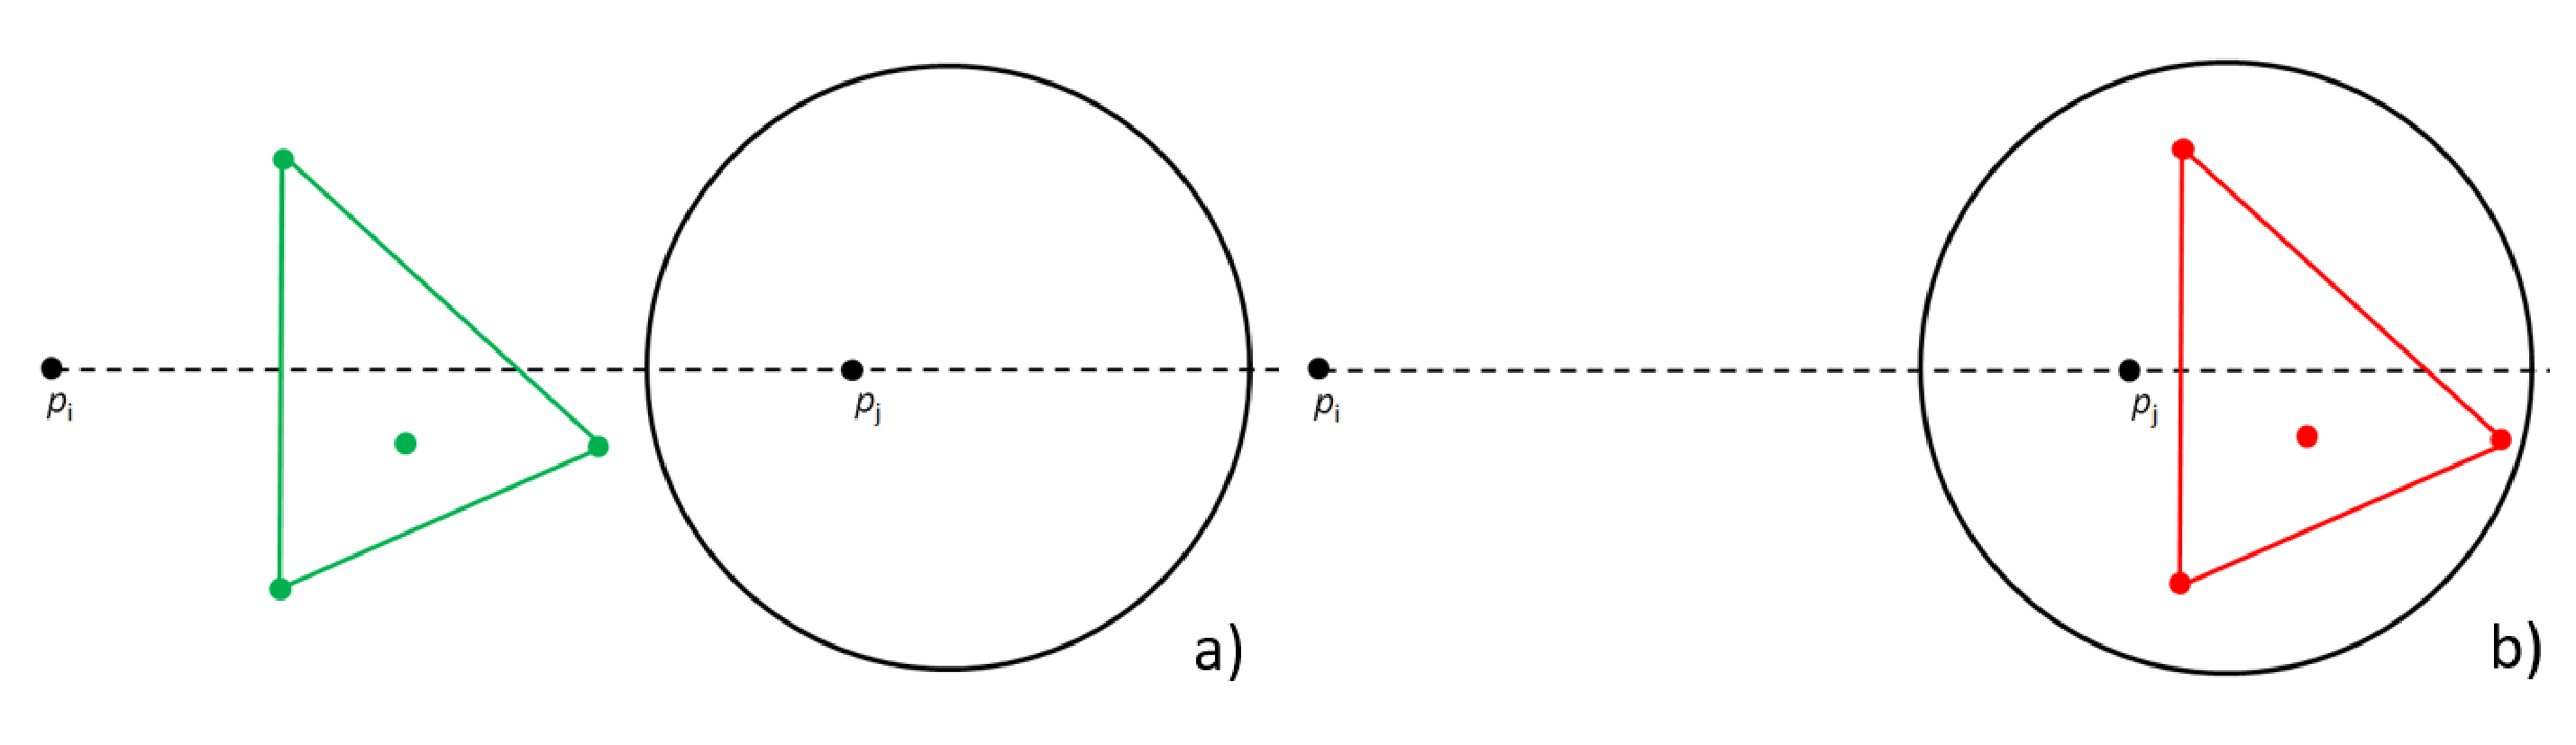
\includegraphics[width=0.8\linewidth]{img/DomNotDom.eps}
%        \caption{a) If $CH(Q) \subset r(p_i, p_j)$ then $p_i$ spatially dominates from near $p_j$ and $p_j$ spatially dominates from far $p_i$; b) If $CH(Q) \subset r(p_j, p_i)$ then $p_j$ spatially dominates from near $p_i$ and $p_i$ spatially dominates from far $p_j$.}
%        %\vspace{-0.5em}
%        \label{fig:DomNotDom}
%        \end{center}
%        \end{figure}

        \vspace{1em}
        \begin{observation} It may be that $E(Q) \subset r(p_i, p_j)$ while $p_i$ does not spatially dominates from near $p_j$, and  $p_j$ does not spatially dominates from far $p_i$.
        \label{obs:w_noCHInrij}
        \end{observation}

         For example, in Figure \ref{fig:NFOnlyE} $E(Q)$ is contained in $r(p_i, p_j)$, but $p_i$ does not spatially dominates from near $p_j$ and $p_j$ does not spatially dominates from far $p_i$.

        \begin{figure}[h]
           \begin{center}
              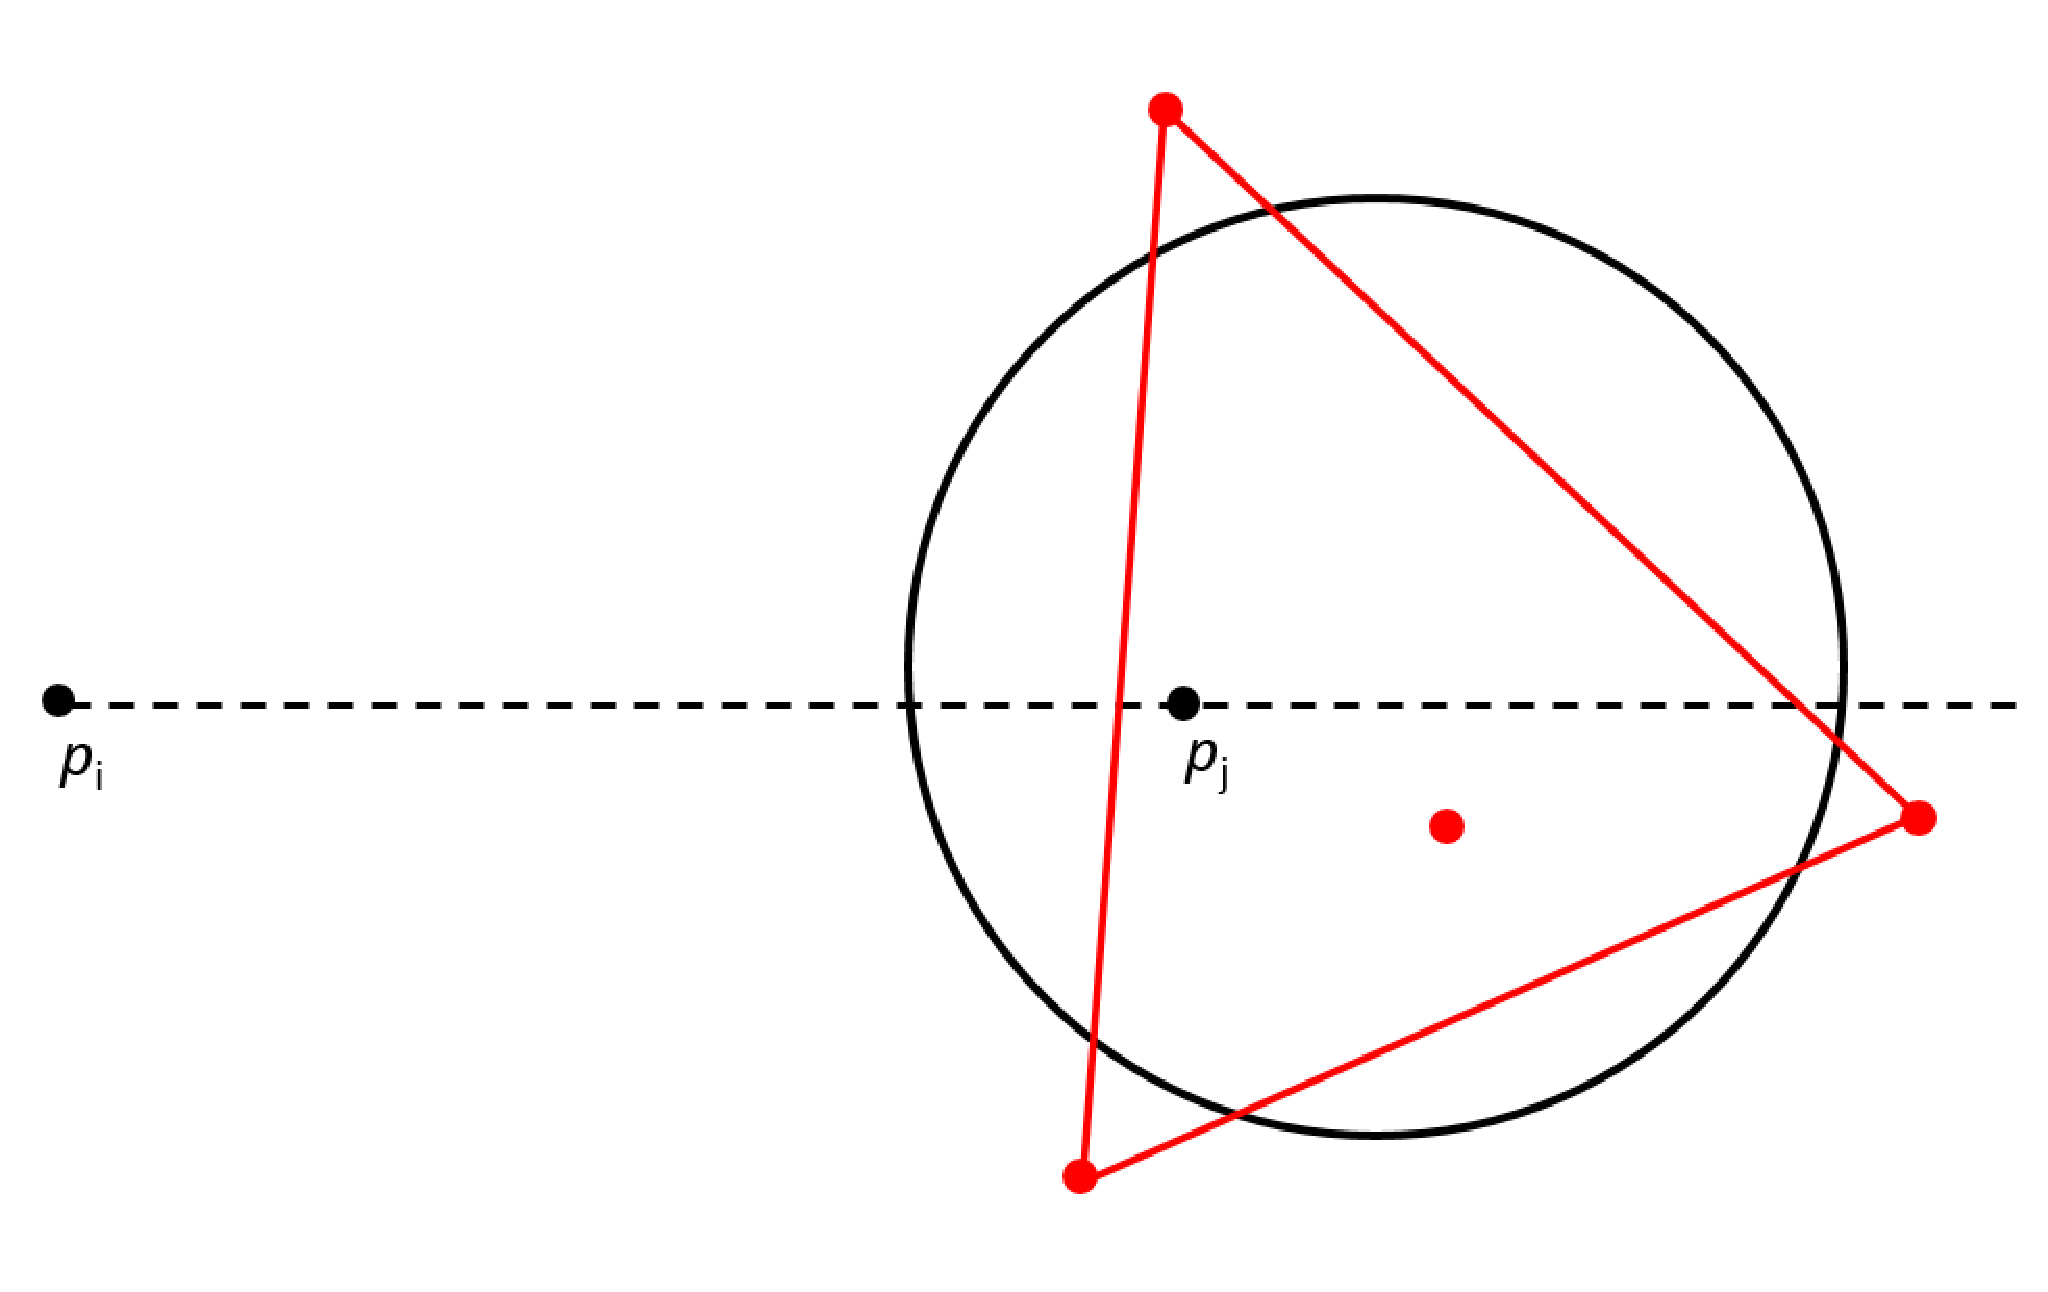
\includegraphics[width=0.4\linewidth]{img/NFOnlyE.eps}
              %\caption{ $E(Q) \subset r(p_i, p_j)$ but $p_i$ does not spatially dominates from near $p_j$; $WSSQ(P,Q)$ does not depend only on $E(Q)$.}
              \caption{Example for Observations \ref{obs:w_noCHInrij} and \ref{obs:w_notCH}}
              \iffalse a) Point $p_i$ dominates from near $p_j$ with respect to $E(Q)$, but $p_j$ is not dominated from near by $p_i$ with respect to $Q$. Point $p_j$ dominates from far $p_i$ with respect to $E(Q)$, but $p_i$ is not dominated from far by $p_j$ with respect to $Q$. b) We have $E(Q) \subset r(p_i, p_j)$, but $p_i$ does not spatially dominates from near $p_j$. We have $E(Q) \subset r(p_i, p_j)$, but $p_j$ does not spatially dominates from far $p_i$.} \fi
              \label{fig:NFOnlyE}
            \end{center}
        \end{figure}


        \vspace{1em}
        \begin{observation} The bisector of two points in $P$ may intersect $CH(Q)$ while one of the weighted points spatially dominates the other from near or does not spatially dominate it from far. \label{observation:w_notBisectorCH}
        \end{observation}

        Next follows an example of each of the two cases. In Figure~\ref{fig:NF_FIntBisectorCH} a) the bisector of $p_i$ and $p_j$ intersects $CH(Q)$, but $p_i$ dominates from near $p_j$. In Figure~\ref{fig:NF_FIntBisectorCH} b) the bisector of $p_i$ and $p_j$ intersects $CH(Q)$, but $p_j$ dominates from far $p_i$.


        \vspace{1em}
        \begin{observation} The set of weighted skyline points of $P$ respect to $Q$ does not depend only on $E(Q)$.
           \label{obs:w_notCH}
        \end{observation}

        For example, in Figure \ref{fig:NFOnlyE} the point $p_i$ dominates from near $p_j$ with respect to $E(Q)$, but $p_j$ is not dominated from near by $p_i$ with respect to $Q$. Point $p_j$ dominates from far $p_i$ with respect to $E(Q)$, but $p_i$ is not dominated from far by $p_j$ with respect to $Q$.

        \vspace{1em}
        \begin{observation} A point of $P$ inside $CH(Q)$ may not be a nearest nor a farthest skyline point.
           \label{obs:w_not_insideCH}
        \end{observation}

        For example, in Figure \ref{fig:NF_FIntBisectorCH} a) the point $p_j$  is inside $CH(Q)$ but it is not a nearest skyline point because $p_i$ dominates it from near. In Figure \ref{fig:NF_FIntBisectorCH} b) the point $p_i$  is inside $CH(Q)$ but it is not a farthest skyline point because $p_j$ dominates it from far.
        \vspace{1em}

         \begin{figure}[h]
          \begin{center}
             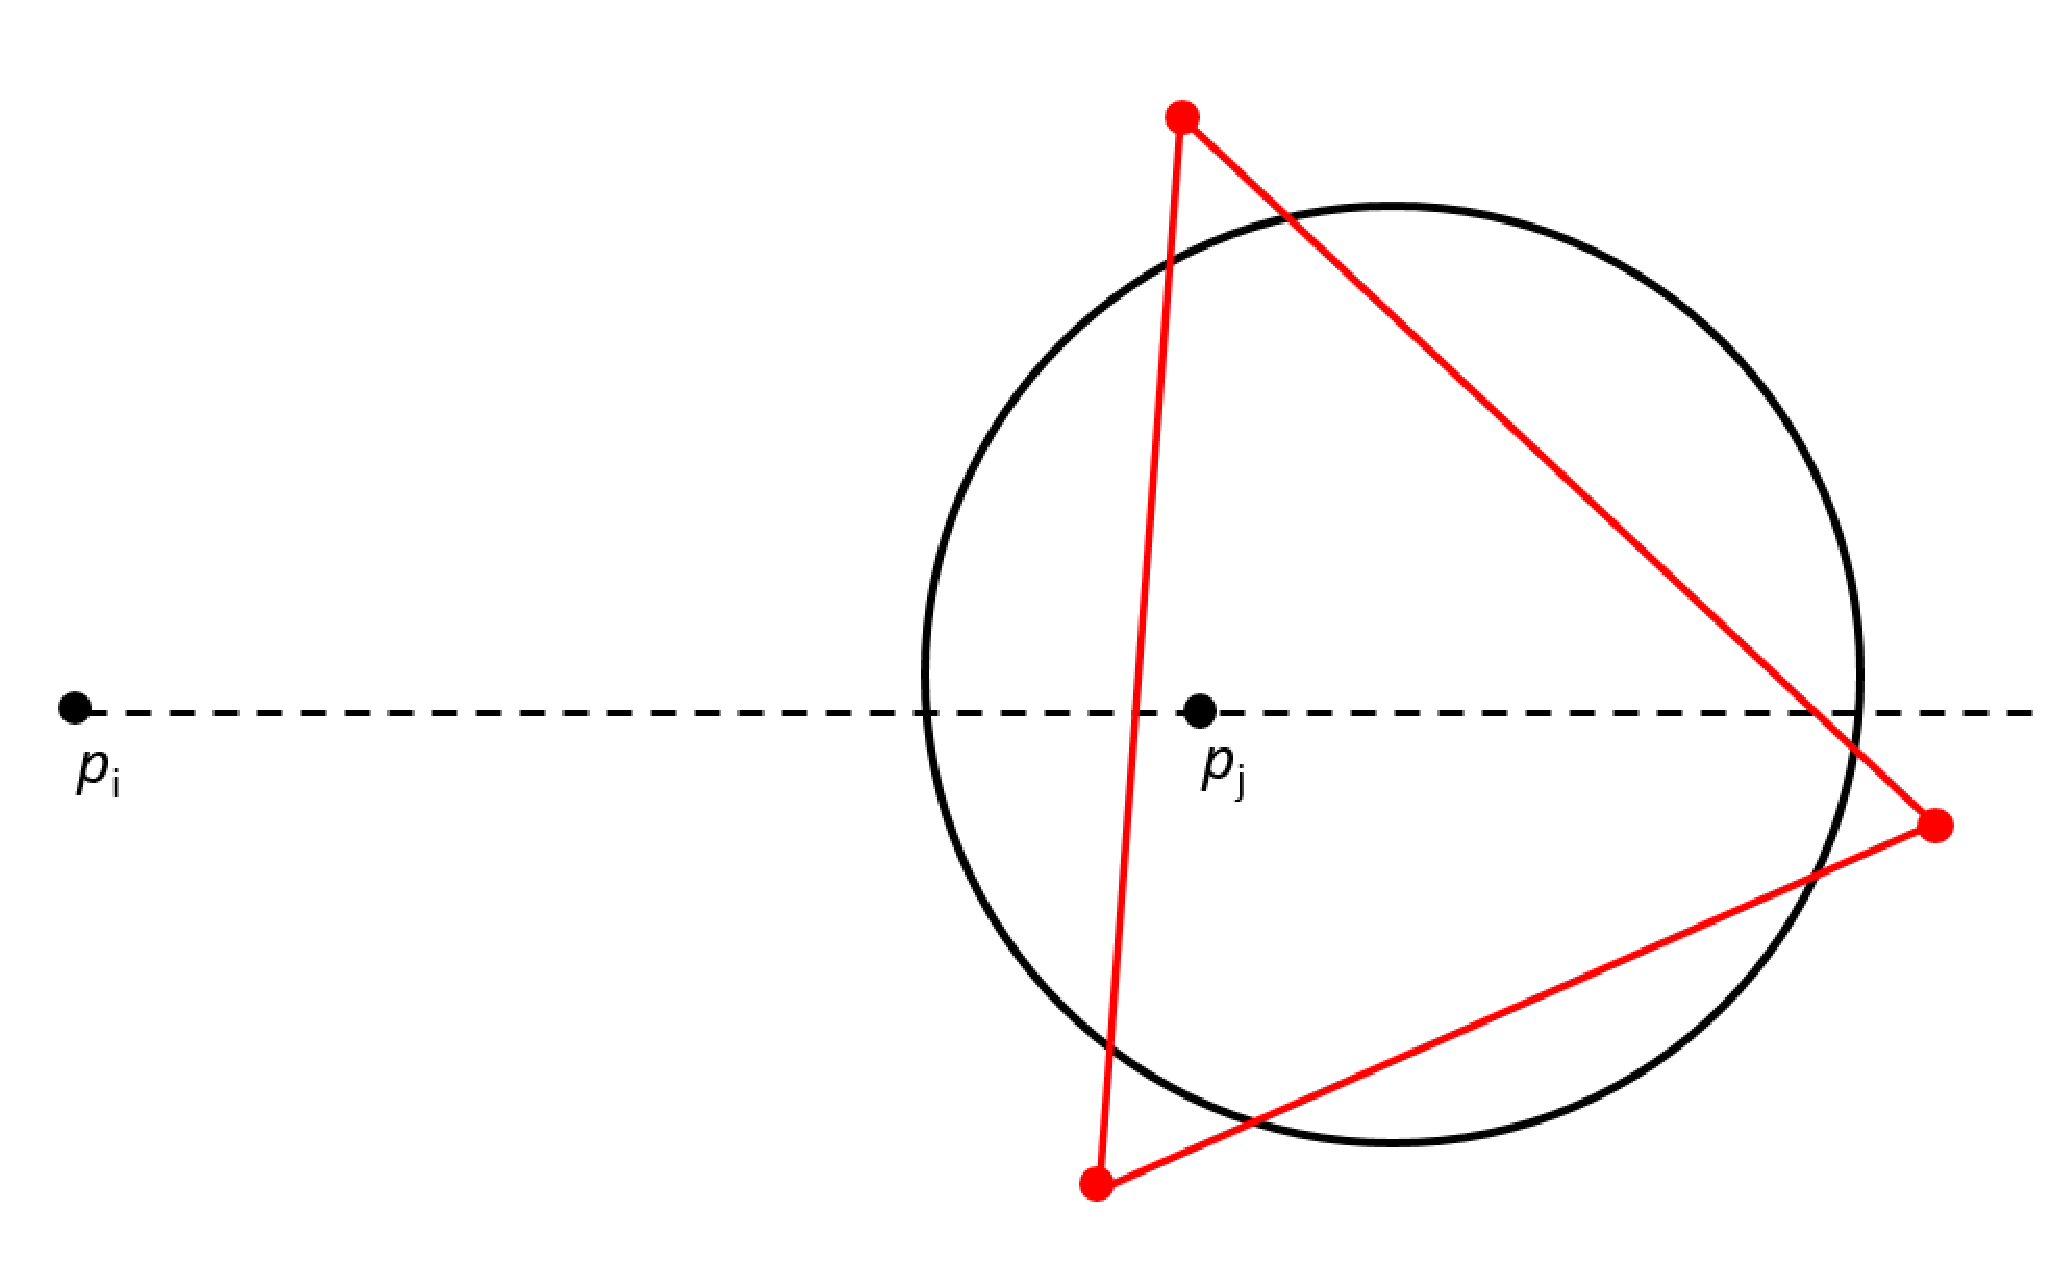
\includegraphics[width=0.4\linewidth]{img/NFIntBisectorCH.eps} a)
             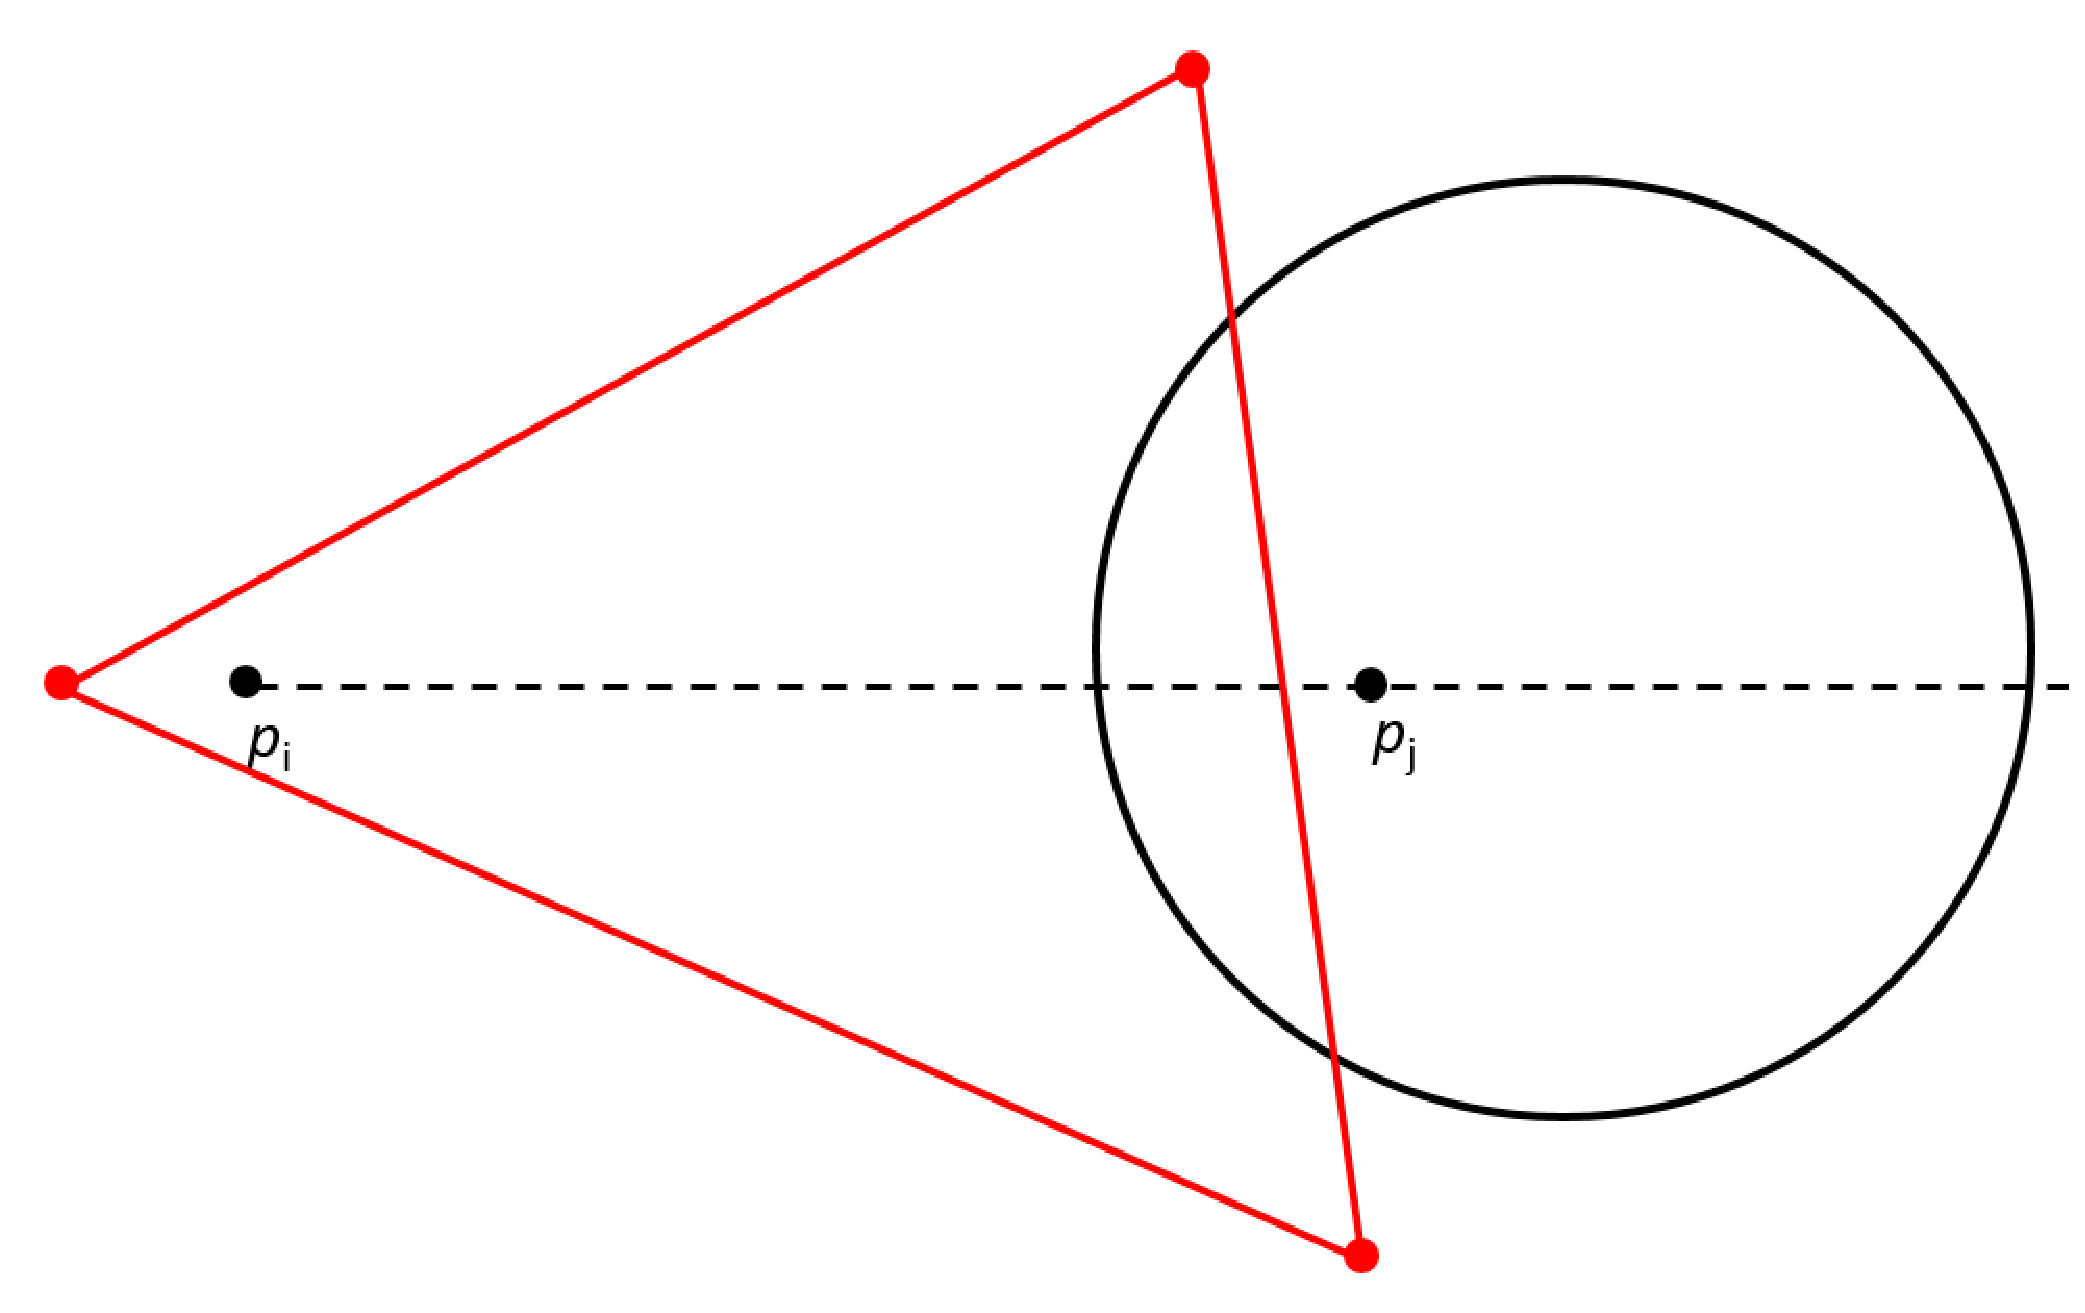
\includegraphics[width=0.4\linewidth]{img/FFIntBisectorCH.eps} b)

             \caption{Examples for Observations \ref{observation:w_notBisectorCH}, \ref{obs:w_not_insideCH} and \ref{obs:w_notVD}: a) from near, b) from far}
             %\iffalse a) From near example: i) The bisector of $p_i$ and $p_j$ intersects $CH(Q)$, but $p_i$ dominates from near $p_j$. ii) Point $p_j$  is inside $CH(Q)$ but it is not a nearest skyline point because $p_i$ dominates it from near. iii) The Voronoi region of $p_j$ intersects with $CH(Q)$ but $p_j$ is not a nearest skyline point because $p_i$ dominates it from near.
             %b) From far example.i) The bisector of $p_i$ and $p_j$ intersects $CH(Q)$, but $p_j$ dominates from far $p_i$. ii) Point $p_i$  is inside $CH(Q)$ but it is not a farthest skyline point because $p_j$ dominates it. iii) The Voronoi region of $p_j$ intersects with $CH(Q)$ and $p_j$ dominates from far $p_i$.
            %}\fif

             \label{fig:NF_FIntBisectorCH}
            \end{center}
       \end{figure}


        \begin{observation}If the Voronoi region of a point of $P$ intersects with $CH(Q)$, the point may not be a nearest skyline point and the point may dominate from far an other point of $P$.
        \label{obs:w_notVD}
        \end{observation}

        In Figure \ref{fig:NF_FIntBisectorCH} a) the Voronoi region of $p_j$ intersects with $CH(Q)$ but $p_j$ is not a nearest skyline point because $p_i$ dominates it from near. b) the Voronoi region of $p_j$ intersects with $CH(Q)$ and $p_j$ dominates from far $p_i$.




        \vspace{1em}
        \begin{lemma} Let $p\in P$ be the closest point to a point $q \in Q$, assuming uniqueness, i.e. $$\forall p' \in P-\{p\} d_p(q)<d_{p'}(q),$$ then $p$ is a weighted spatial skyline point from near.\label{lemma:w_closestWSS} \end{lemma}
         \vspace{1em}

         \vspace{1em} \begin{lemma} Let $p\in P$ be the farthest point to a point $q \in Q$, assuming uniqueness, i.e. $$\forall p' \in P-\{p\} d_p(q)>d_{p'}(q),$$ then $p$ is a weighted spatial skyline point from far. \label{lemma:w_farthestWSS} \end{lemma}
         \vspace{1em}

         \begin{lemma} {\it $[$Transitivity$]$} If $p_i$ spatially dominates $p_j$ and $p_j$ spatially dominates $p_k$; then $p_i$ spatially dominates $p_k$. \vspace{0.6em} \label{lemma:w_transitivity}\end{lemma}
       % \begin{proof} Since $p_i$ dominates $p_j$ and $p_j$ dominates $p_k$ $\forall q_l\in Q$  $d_{p_i}(q_l) \le d_{p_j}(q_l) \le d_{p_k}(q_l)$ and $\exists q_r\in Q$ with $d_{p_i}(q_r) < d_{p_j}(q_l) \le d_{p_k}(q_l)$ and hence $p_i$ dominates $p_k$. \end{proof}

         We do not provide the profs of the lemmas because they are trivial and are an adaptation of those for the unweighted case.



\subsection{Unweighted versus weighted spatial skyline queries comparison}

Many of the properties used to solve unweighed spatial skyline queries are not further true when weights are associated to the points of $P$. Figure~\ref{fig:propertiesSummary} provides a summary of the properties of the nearest and farthest spatial skyline problems for both the unweighed and weighted problem. It also summarizes the properties used in each of the existent algorithms to determine the unweighted skyline points.

        \begin{figure}[h]
        \begin{center}
        
\includegraphics[width=\linewidth]{img/summary.eps}
        %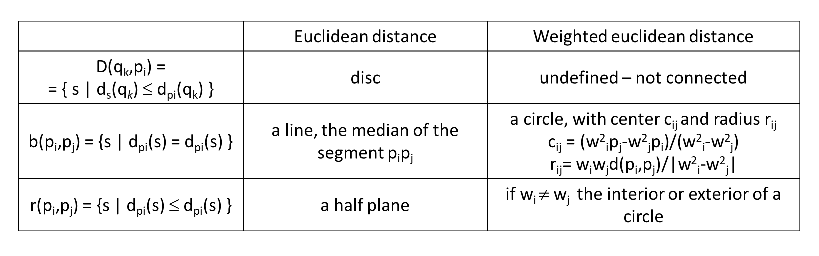
\includegraphics[width=0.6\linewidth]{img/summary_regions.eps} a)
        %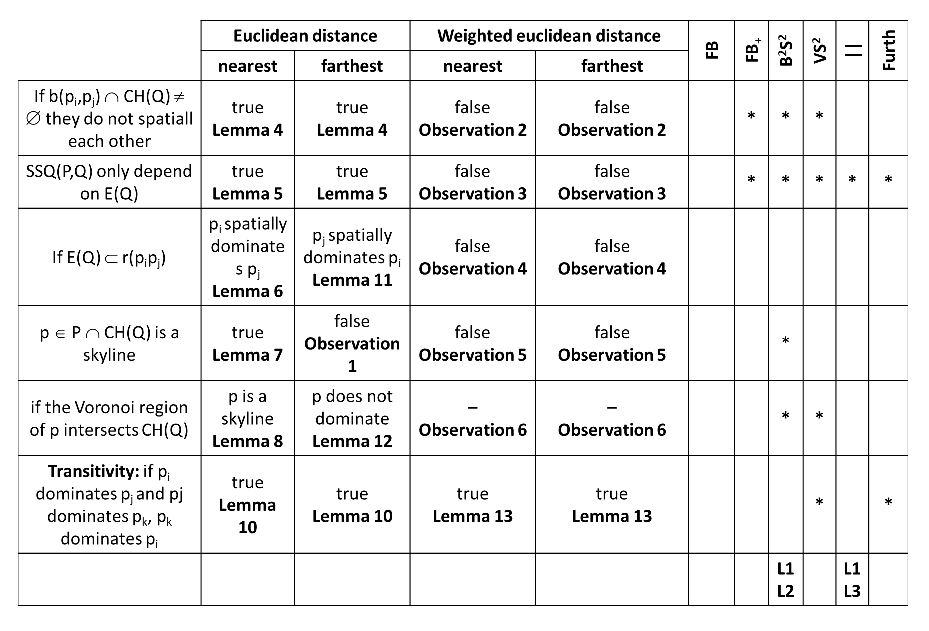
\includegraphics[width=0.8\linewidth]{img/summary_properties.eps} b)
        \caption{Geometric properties and algorithms summary }
        %c) The Voronoi region of $p_j$ intersects with $CH(Q)$ and $p_j$ dominates from far $p_i$.
        \label{fig:propertiesSummary}
        \end{center}
        \end{figure}

According to the observations related to the weighted spatial skyline points, neither the convex hull nor the Voronoi diagrams can be used to accelerate the weighted skylines determination. On the contrary, the properties related to the search and dominator regions are still true. However, meanwhile under the unweighted Euclidean distance they are unions or intersections of circles and they are easy to be approximated or bounded, under the weighted distance they turned to be defined by circular arcs and may have several disconnected components. Their irregular shapes make them difficult or impossible to bound or approximate.  Moreover, in the unweighted case, several data structures are used to reduce the number of dominance tests, but the properties allowing their use mainly rely on the triangular inequality that is no longer true when weights are considered. Finally, there also exist several properties used in the unweighted case that are proven by considering an arbitrary point in $\mathbb{R}^2$ and assuming that it is a point of $P$. These proves can not be generalized to the weighted case, an arbitrary point $p\in \mathbb{R}^2$ can not be a point of $P$, the weight is missing and it can not be arbitrarily chosen because its value notoriously affects results. Hence, many of the proved results and strategies used for the unweighted case are not generalizable to the weighted case.

In fact, as it can also be seen in Figure~\ref{fig:propertiesSummary}, most of the existent algorithms use properties to avoid the dominance tests and accelerate the unweighted skyline points determination that can not be used with the weighted Euclidean distance. The two basic properties that are used in all the algorithms, the reduction of $Q$ to $E(Q)$ and answering the dominance test by checking whether $b(p_i,p_j)$ intersects $CH(Q)$, can not longer be used. By analysing the algorithms, from left to right according to the table, we see that the properties used in $BF$ are extended to the weighted case, $BF$ is adaptable to the weighted scenery, but it is not true for the accelerated version $ABF$. In its turn, $B^2S^2$ and $VS^2$ are not adaptable because their accelerations relay on the geometric shape of the search and dominator regions which can no longer be easily determined or bounded. On the contrary, the fastest known sequential algorithm, $DS$, apart from simplifying the problem by using $E(Q)$, only uses the transitivity of the dominance relation, which still holds. The next algorithm, $PA$, is based on the triangular inequality of the Euclidean distance which is not fulfilled and, hence, it can not be adapted to the weighted case. Finally, $BBFS$ uses the shape of the search regions to accelerate the process, which makes it not adaptable to the weighted case neither. % Hence, the only algorithms that can be extended to solve the weighted spatial skyline problem are the $DS$ and $BF$ using the whole set $Q$ and the definition to perform the dominance tests. %Finally, note that the force brute algorithm can be almost fully parallelized, meanwhile $DS$ is a completely sequential algorithm, it basically exploits its sequentiality to reduce the dominance tests to the already determined skyline points. These are the two algorithms that we adapt to the weighted case in next section.

The fact that most of the properties and algorithms can not be extended to the weighted case is not that surprising because the nature of the problems are completely different. The weight makes that each point of $P$ derives to $|Q|$ virtual points. Each point $p\in P$ is virtually placed at a different location for each query of $Q$. This is represented in Figure~\ref{fig:virtual_location} where the set of points $P$ is virtually transformed to $\{p_{1,j}, p_{2,j}\}$ according to each $q_j\in Q$.


        \begin{figure}[]
        \begin{center}
        
\includegraphics[width=0.3\linewidth]{img/P3_q2.eps}
        \caption{ $P=\{p_1,p_2\}$ is virtually transformed to $\{p_{1,j}, p_{2,j}\}$ according to $q_j\in Q = \{q_1, q_2, q_3\}$}\label{fig:virtual_location}
        %c) The Voronoi region of $p_j$ intersects with $CH(Q)$ and $p_j$ dominates from far $p_i$.
        \end{center}
        \end{figure}




\section{Weighted spatial skyline obtention} \label{sec:Algorithms}

    In this section, we present the algorithms to solve the weighted spatial skyline problem. As we mentioned before, apart from solving the problem sequentially in the CPU we also want to take advantage of the parallel and compute capabilities of the GPU to accelerate the process. In fact, the GPU has been used in last years to accelerate the resolution of many problems and it is shown that it provides very good results \cite{FS13,FS14a,FS15,FS16, FS16b,XW18,XZCMW18}. Hence, we want to exploit its parallel and compute capabilities to try to solve the problem faster in parallel.

    In order to accomplish both objectives, we first present $WDS$ the sequential algorithm which is an adaptation of the $DS$ algorithm to the weighted Euclidean distance and second our $PWBF$ parallel proposal which is based on the $BF$ algorithm. Then, the algorithms are theoretically analyzed and compared in terms of time and space complexity.

    \subsection{Sequential algorithms} \label{sec:seq_alg}

        We present the $WDS$ algorithm which starts sorting the points of $P$ according to their weighted distance to an arbitrarily chosen point $\tilde{q}\in Q$. If we solve the problem {\it from-near}, the points of $P$ are sorted by increasing distance to $\tilde{q}$, so that, after sorting, for every $p_i, p_j\in P$, $d_{p_i}(\tilde{q}) \le d_{p_j}(\tilde{q})$ whenever $i < j$. Meanwhile, when solving the problem {\it from-far} they are sorted by decreasing distance order, so that, once sorted, $d_{p_i}(\tilde{q}) \ge d_{p_j}(\tilde{q})$, whenever $i < j$.

        Then, according to Lemmas~\ref{lemma:w_closestWSS} and~\ref{lemma:w_farthestWSS}, the first point of $P$ is stored at $SSWQ$ for being a spatial skyline. Next, we analyze the points of $P$ per order, because Lemma~\ref{lemma:w_transitivity} guarantees that any not-skyline point $p_i$ will be dominated by one of the already detected skyline points $p_j$ with $j<i$. Hence, for each point $p_i \in P$ we check whether it is dominated by any of the already detected skylines. If it is not dominated by any of them, it is a skyline point and it is stored at $SSWQ$. See Figure~\ref{fig:alg_seq} for the pseudo-code of the algorithm.

         \begin{figure}[h]
            \begin{center}
            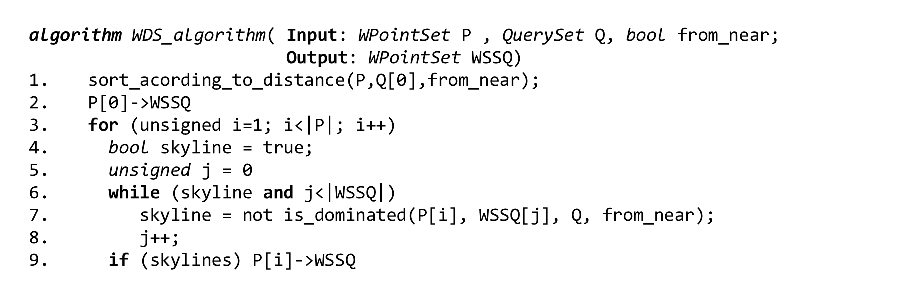
\includegraphics[width=0.75\linewidth]{img/algorithm_DS.eps}
            \caption{ $WDS$ sequential algorithm pseudocode}\label{fig:alg_seq}
            %c) The Voronoi region of $p_j$ intersects with $CH(Q)$ and $p_j$ dominates from far $p_i$.
            \end{center}
         \end{figure}

        To check whether point $p_i \in P$ is dominated by point $p_j \in SSQ$, we perform the dominance test according to the definition. Hence, we look for a query $\overline{q}\in Q$ closer to, or farther from, $p_i$ than to $p_j$, depending on whether we solve the problem {\it from-near} or {\it from-far}. Such a query $\overline{q}$ ensures that $p_i$ is not dominated by $p_j$. If $\overline{q}$ does not exist, $p_j$ dominates $p_i$ and $p_i$ is not a skyline. See Figure~\ref{fig:alg_DomTest} for the pseudocode of the dominance test.

         \begin{figure}[h]
            \begin{center}
            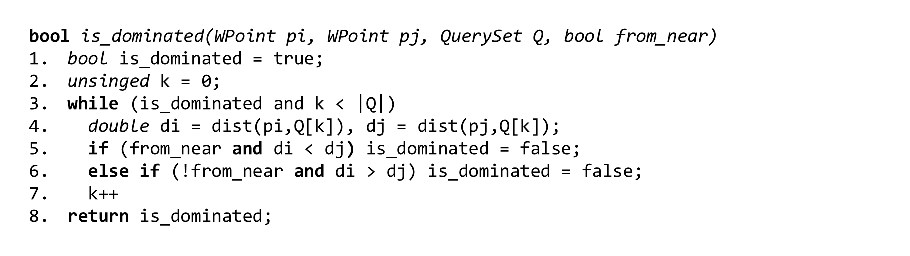
\includegraphics[width=0.75\linewidth]{img/algorithm_DT.eps}
            \caption{Dominance test pseudocode}\label{fig:alg_DomTest}
            %c) The Voronoi region of $p_j$ intersects with $CH(Q)$ and $p_j$ dominates from far $p_i$.
            \end{center}
         \end{figure}


         \vspace{1.5em}

        \noindent {\bf Complexity analysis.}  As before, we denote $n=|P|$, $m=|Q|$ and $r=|SSQ(P,Q)|$. Accordingly, the memory requirements of this strategy are $O(n+m+r) = O(n+m)$. Concerning the time complexity of the $WDS$ algorithm, it takes $O(n\log n)$ time to sort $P$ with respect to the distance to $\tilde{q}\in Q$. Determining the skylines requires performing, in the worst case, $O(nr)$ dominance tests, taking $O(m)$ time each. Hence, the worst case time complexity of this algorithm is in $O(nlogn + nmr)$. Since $r = \Omega(n)$, in the worst case it becomes $O(n^2m)$ and equals the time complexity of the force brute algorithm. On the other hand, in the best case, after sorting $P$ in $O(n\log n)$ time, it performs $O(n)$ dominance tests with $O(1)$ work each, which gives a best case time complexity of $WDS$ of $O(n\log n)$.

        %Notice that $O(n^2m)$ is the worst case complexity of the brute force algorithm. The force brute algorithm determines wether a point $p_i\in P$ is a skyline point by performing $O(n)$ tests, one per point $p_j\in P - \{p_i\}$. Consequently the brute force pseudocode differs from that in Figure~\ref{fig:alg_seq} in lines $6.$ and $7.$, in this case $j <= |P|$ and that the dominance test is done with $P[i]$ and $P[j]$.

    \subsection{Parallel algorithm} \label{seq:paral_alg}

        When we looked for a parallel algorithm to solve the problem, we found several strategies to tackle the problem in parallel. We designed, implemented and tested the parallel algorithms that we could design and we present, in this section, the best algorithm, among the analyzed ones, in terms of running times and sketched in Section~\ref{sec:ExpResultsDis} the discarded ones.

        %The $PWBF$ algorithm is a parallelization of the brute force algorithm. In fact, there exist several ways to parallelize it, if we try to parallelize as much as we can, we would consider one thread per triplet $(p_i,p_j,q)\in P\times P\times Q$, and the thread would simply compare de distances $d_{p_i}(q)$ and $d_{p_j}(q)$, but we would need too much threads and since the number of threads and we would not explode the compute capabilities of the GPU. We could also consider one thread per pair $(p_i, p_j) \in P\times P$ so that each thread checks whether $p_i$ is dominated by $p_i$ by analysing the $|Q|$ queries. In this case the number of required threads would be $|P|^2$ which is still huge and we would have $|P|$ threads analyzing whether $p_i$ is a skyline and any of them could decide at any time that it is not a skyline and the rest would be doing nonsense computations. Finally, what we do is considering a single thread per point $p\in P$ and it determines whether $p \in WSSP$. The thread would perform at most $|P|$ dominance tests analyzing at most $|Q|$ queries each. This last strategy is the one taking much benefit of the parallel capabilities of the GPU, we could also take advantage of its memory structure and avoid unnecessary computations, as soon as a point is dominated the thread knows it and stops analyzing other points of $P$.\\

        The best parallel algorithm, $PWBF$, is a parallelization of the brute force algorithm that uses a single kernel and considers a thread per point $p\in P$ to determine whether it is a skyline point. In fact, before calling the kernel, whose pseudocode is presented in Figure~\ref{fig:alg_paral}, we transfer $P$ to a GPU global memory array $hP$ and $Q$ to a GPU constant memory array $chQ$. The kernel uses $hS$, an integer uninitialized array of size $n$, to store the output. Array $hS$ is stored in global memory and ends with a $1$ or a $0$ in its position $S[i]$, depending on whether point $P[i]$ is or is not a skyline. Once the kernel has finished, array $hS$ is transferred to a CPU array $S$ which is traversed while copying the points $P[i]$ with $hS[i]$ equal to $1$ to $SSWQ$.


        \begin{figure}[]
        \begin{center}
        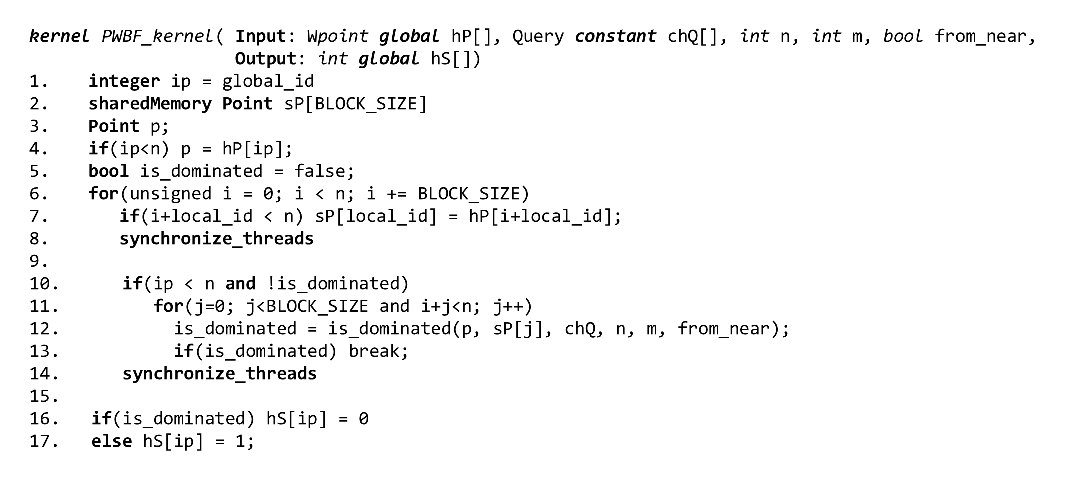
\includegraphics[width=0.9\linewidth]{img/algorithm_PA.eps}
        %
\includegraphics[width=0.3\linewidth]{img/P3_q2.eps}
        \caption{PWBF algorithm pseudocode}\label{fig:alg_paral}
        %c) The Voronoi region of $p_j$ intersects with $CH(Q)$ and $p_j$ dominates from far $p_i$.
        \end{center}
        \end{figure}


        When the kernel is executed each thread is responsible of a point in $hP$, in fact the thread with global identifier $id$ determines whether the point $p_{id} = P[id]$ is a skyline point. It starts by analyzing the rest of points of $hP$ until, either all the points have been analyzed, or it finds a point $p_j\neq p_{id}$ that dominates $p_{id}$. Since it is known that point $p_{id}$ is not a skyline as soon $p_{id}$ is dominated, in such a case, the thread stops analyzing points of $P$ and sets $hS[id]$ to $0$. If all the points of $P$ are analyzed and $p_{id}$ has not been dominated, it is marked as a skyline point by setting $hS[id]$ to $1$. The dominance test associated to $p_j$ and $p_{id}$ is performed in the GPU using an algorithm analog to the one presented for the WSD algorithm whose pseudocode is provided in Figure~\ref{fig:alg_DomTest}. However, now the queries are obtained from the GPU constant memory array $chQ$.

        Finally, we want to mention that since all the threads potentially traverse the whole set $hP$ to determine whether their point $p_{id}$ is a skyline, the threads in a block cooperate to transfer $hP$ to shared memory in blocks of BLOCK\underline{ }SIZE size. It implies using two synchronization points, one after the kernel transfers a point of $hP$ to shared memory and the other after the thread has finished analyzing the points stored in shared memory. Note that, it makes that those threads that had already determined that their associated point is dominated have to keep on transferring points to shared memory. However, they will not analyze them.

\vspace{1.5em}

        \noindent {\bf Complexity analysis.} Concerning the memory requirements, the PWBF algorithm stores $P$ and $hS$ in global memory, $P$ is transferred to shared memory and $Q$ is stored to constant memory. Hence it uses $3n$ real values an $n$ integer values in global memory, $2n$ real values in constant memory and we use $2 BLOCK$\underline{ }$SIZE$ real values of shared memory per block, i.e. it uses $O(n+m)$ memory in the GPU. In the CPU we store $P$, $Q$ and $WSSQ$, i.e. it requires $O(n+m+r)=O(n+m)$ memory.

        To perform its time complexity analysis, since it is a parallel algorithm, we analyze the {\it worst case total work} done by the algorithm and the {\it execution time of the algorithm} when $p$ threads are used. The worst case total work is the number of executed operations over all the processors or threads. In this algorithm we use $n$ threads and each thread does $O(nm)$ work in the worst case. The sequential part of the algorithm which traverses $S$ to determine $WSSQ$ does $O(n)$ work. Hence, the total work done by the algorithm in the worst case is $O(n^2 m)$. Meanwhile, the execution time of the algorithm when $p \in O(n)$ threads are considered is of $O(n^2m/p)$. Concerning the best case analysis, each thread does $O(1)$ work, the total work would be $O(n)$, which would be done by $p=O(n)$ threads. This provides an execution time of $O(n/p)$.

\subsection{Theoretical comparison between the parallel and sequential algorithm}
        By comparing the complexities of the parallel and sequential presented strategies, we can see that the total work done in the worst case for the sequential WSD algorithm is output-dependent, meanwhile that of parallel PWBF algorithm is independent from the output. Hence, in general, the total work complexity of the PWBF algorithm is worse than that of the WSD, meanwhile concerning the execution time there is no so much difference. Moreover, in the case that the output is as big as possible, both complexities coincide and hence the execution time of the PWBF algorithm is much better than that of the WSD.\\


        Apart from this initial observation, the standard measures to theoretically compare a parallel and a sequential algorithm are the parallel speedup and the work efficiency of the parallel algorithm. They refer, respectively, to the time complexity $t$ of the best known sequential algorithm to solve the problem, which is $WSD$, and the execution time $t_p$ and the total work $w$ of the parallel algorithm, $PWBF$. Next we use these measures to compare WSD and PWBF.\\

        \begin{description}

            \item[Work efficiency:] it is defined as the ratio $\frac{w}{t}$, which in our case is  $$\frac{w}{t} = O(n^2m/rnm) = O(n/r).$$ It reflects that PWBF does more work than the  WSD, which is due to the fact that WSD is output dependent and PWBF is not.\\

            \item[Theoretical parallel speedup:] it is given by the ratio $\frac{t}{t_p}$, which in our case is $$\frac{t}{t_p} = O\left(\frac{rnm}{\frac{n^2m}{p}}\right) = O\left(\frac{p\ r}{n}\right).$$
                Again, the extra work done by PWBF algorithm penalises it. Even enough this ratio would generally be greater than 1 and PWBF would theoretically perform better than WSD,  for very small outputs it would be smaller than 1, which would mean that WSD algorithm would perform better than PWBF.\\

            \item[Space complexity comparison:] The space complexity of both algorithms is $O(n+m)$. Thus, the space complexity of the parallel algorithm is optimal.\\

        \end{description}

        Accordingly, even though the PWBF parallel algorithm does more work than the sequential WSD one, since it proceeds in parallel, it will perform better than WDS except for cases in which too small outputs, in percentage, were obtained. %s running times are much better as it is shown in Section~\ref{sec:ExpResults}.


\section{Top-$k$ skylines}\label{sec:top_k}
        Sometimes, as it happens with the traditional spatial skylines, after determining the skylines there are still too many desirable points to choose among, in these cases,  extracting the top-$k$ or the best $k$ ones is useful. Hence, we want to allow the user to provide a $k$ value and to extract the best $k$ skylines according to a scoring function that can be chosen among the ones presented in Section~\ref{sec:Background}. % $$\delta_{max}(p) = \max_{q \in Q} d_p(q); \;\; \delta_{min}(p) = \min_{q \in Q} d_p(q)  \; \text{ and } \delta_{sum}(p) = \sum_{q \in Q} d_p(q).$$
        The top-$k$ skylines are those minimizing the scoring function in the from near case and those maximizing it in the from far case.

        If the user decides to determine the top-$k$ skylines once the skylines have already been obtained, using the GPU makes no sense. In this case we evaluate, in the CPU, the scoring function and maintain its top-k values and the skylines achieving them. However, if the user starts asking for the the top-$k$ spatial skyline points, the process can be accelerated by computing the value of the scoring function in parallel in GPU. It is computed during the skylines detection by slightly modifying the PWBF algorithm according to Figure~\ref{fig:alg_paral_topk}, where we provide the Top-$k$ PWBF algorithm pseudocode. In the Top-$k$ PWBF algorithm, each thread determines whether its associated point of $P$ is a skyline point and, when it is a skyline, it evaluates the scoring function. It is done by traversing $Q$ and determining the distances from the queries to the already detected weighted spatial skyline point. The output is now a real array  which stores in the $i$-th position a $-1$ when $P[i]$ is not a skyline and the value of the scoring function when it is a skyline. This real output array is transferred to the CPU where it is traversed while the top-$k$ values and the positions with o non -1 value are determined. The weighted points occupying these positions are also stored for being the desired top-$k$ weighted skyline points.

        \begin{figure}[]
        \begin{center}
        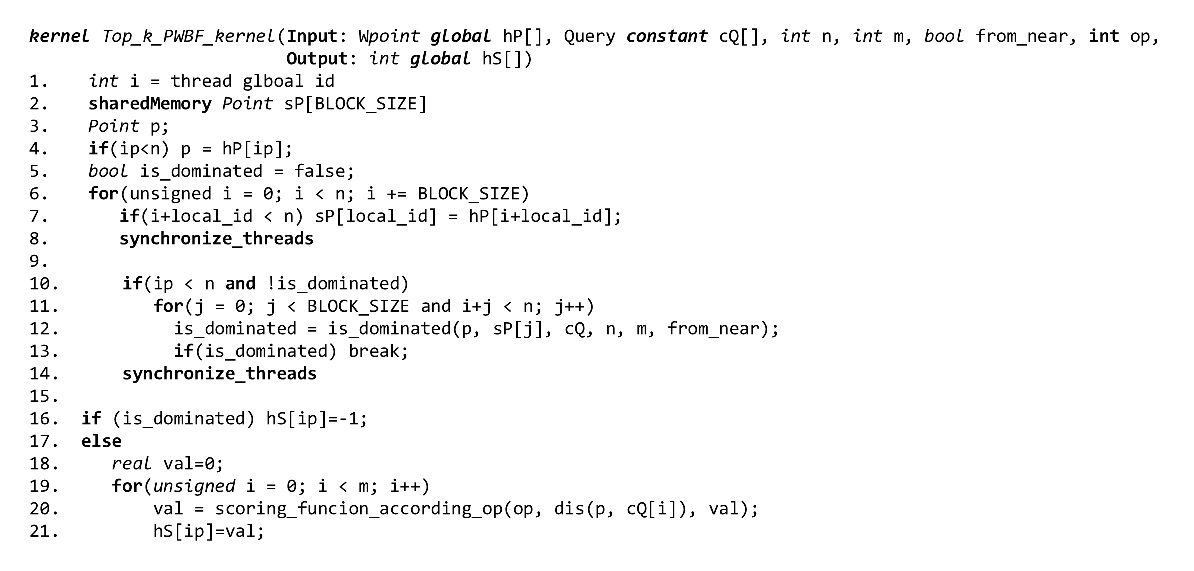
\includegraphics[width=\linewidth]{img/algorithm_PA_tk.eps}
        %
\includegraphics[width=0.3\linewidth]{img/P3_q2.eps}
        \caption{Top-$k$ PWBF algorithm pseudocode}\label{fig:alg_paral_topk}
        %c) The Voronoi region of $p_j$ intersects with $CH(Q)$ and $p_j$ dominates from far $p_i$.
        \end{center}
        \end{figure}
\vspace{1.5em}

        \noindent {\bf Complexity analysis.} Determining the top-$k$ weighted spatial skylines once the $r$ weighted spatial skylines have been detected requires $O(rm)$ time to evaluate the scoring function and $O(r\log k)$ time to determine the top $k$ ones, i.e. $O(rm + r\log k)$ extra time. This can be done with $O(k)$ extra space, or with no extra space if desired.

        Concerning the Top-$k$ PBF algorithm, each thread does $O(m)$ extra work. Since the work needed to determine the skyline points is $O(nm)$, obtaining the value of the scoring function does not increment the order of complexity of the work done by the threads. Hence, the complexity analysis of the parallel part of the algorithm does not change. We have to add the time needed to obtain the top-$k$ values in the CPU which is $O(n\log k)$ extra time. Hence, the total work done by this algorithm is $O(mn^2+n\log k)$ and when $p\in O(n)$ threads are used the execution time becomes $O(mn^2/p+n\log k)$.  Concerning the extra space, it can be done without extra space or using at most $O(k)$ extra space.

\section{Experimental results}\label{sec:ExpResults}

This section is subdivided in three subsections. First, we present the interface we developed to deal with the weighted skylines problem. Then, we analyse the running time performance of the presented algorithms. Finally, we briefly discuss several explored, implemented and tested ways to solve the problem that were discarded due to their performance.

All the implementations have been done in C++, for the parallel part Cuda C has been used and the visualization is done by using OpenGL.


\subsection{Results visualization}
 We have developed an interface to deal with the weighted spatial skyline problem. This allows to easily obtain, visualize and store the sets $P$, $Q$ and $WSSQ$. Sets $P$ and $Q$ can be read from a {\it .json} and {\it binary} files, placed manually or generated randomly. The user can zoom-in and out with the mouse and also select any of the points to edit it modifying its coordinates or weight. The set $WSSQ$ is computed once all the parameters are specified. If desired, the used data and the obtained WSSQ set can be stored in {\it .json} or {\it binary} files.

 As it is shown in Figure~\ref{fig:w_Images} queries are colored in blue, the weighted points are gradated in red according to their weight (the darker the smaller the weight) and the obtained skylines remarked with a green background. In this case, the set $P$ has 1000 weighted points and $Q$ 50 queries, the nearest and farthest skylines are remarked with the green square in the first row and the top-$10$ ones in the second one. Note that the images reflect that not all the points in the convex hull of $Q$ are weighted skyline points, that the nearest skylines tend to be not too far from the points of $Q$ and that the farthest ones are either close to the {\it center} of $Q$ or to the boundaries of $P$.
 \begin{figure}[]
        \begin{center}
          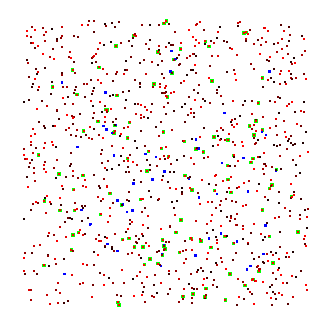
\includegraphics[width=0.33\linewidth]{img/random_1000_50_nearest_all.eps} a) \qquad
          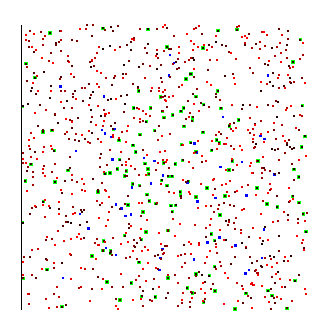
\includegraphics[width=0.33\linewidth]{img/random_1000_50_furthest_all.eps} b)\\
          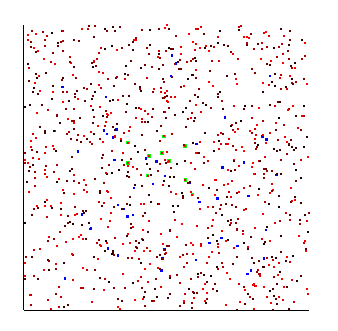
\includegraphics[width=0.33\linewidth]{img/random_1000_50_nearest_top_10.eps} c) \qquad
          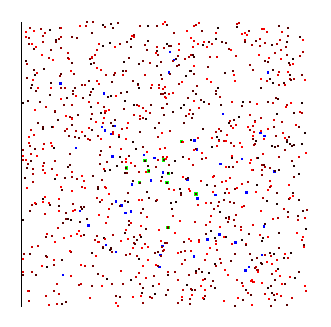
\includegraphics[width=0.33\linewidth]{img/random_1000_50_furthest_top_10.eps} d)\\
            Nearest \hspace{0.33\linewidth}  Farthest
          \caption{In red 1000 weighted points, in blue 50 query points, in green all the skylines in a) and b), the top-10 in c) and d)
          }\label{fig:w_Images}
        \end{center}
     \end{figure}

  In Figure~\ref{fig:bcn_region} $P$ is defined by $379$ points corresponding to the locations of the hotels of the seaside city of Barcelona (in the south-west of Europe) that are registered at OpenSteetsMap, a collaborative project to create a free editable map of the world, \cite{OpenStreetMap} in july 2018. We considered the hotels with latitud between 2.100 and 2.25 and longitud between 41.38 and 41.44. \iffalse which correspond to the hotels in the region represented in the left of the image a).\fi \iffalse which corresponds to the region represented in Figure~\ref{fig:bcn_region}. \fi In the images of the first row, the set of queries $Q$ is defined by 9 tourist places of Barcelona: {\it El Born, Sagrada Familia, La Pedrera (Gaudi house), El Liceu, Mafre Tower, Agbar Tower, The Cathedral, Tibidabo} and {\it Montju\"ic Castel} which are displaced along the whole city. The images correspond, from left to right, to all the nearest skyline points, the top-5 ones and all the farthest skyline points. We do not extract the 5-top farthest skylines because there only exist 8 points in c) and 3 in f). Concerning the top-5 nearest ones, somehow, one could expect that the top-5 ones where selected closer to the city center, where the density of hotels is greater. However, they are quite displaced to the left due to the query point placed al the top-left corner of the image, which corresponds to {\it Montju\"ic Castel}. In the second row, we solved the same problems after eliminating  {\it Montju\"ic Castel} from $Q$. In this case, the nearest skylines and the top-5 ones are mainly in the center of the city which is also the center of $Q$. Meanwhile there disappear the furthest skylines that were located in the city center that are present in the image of the first row. %This set $Q$ could be used for the from near case but it could also be used for the from far case if one is interested in avoiding the typically visited places of the city.

    \begin{figure}[]
        \begin{center}
%          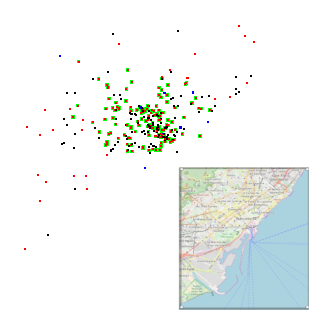
\includegraphics[width=0.3\linewidth]{img/bcn_nearest_all_bcn.eps} a)
          \includegraphics[width=0.3\linewidth]{img/bcn_nearest_all.eps} a)
          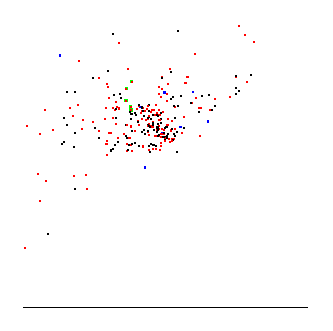
\includegraphics[width=0.3\linewidth]{img/bcn_nearest_top5.eps} b)
          
\includegraphics[width=0.3\linewidth]{img/bcn_farthest_all.eps} c)
%          \includegraphics[width=0.3\linewidth]{img/bcn_area_2.eps} d)
          \includegraphics[width=0.3\linewidth]{img/bcn_nearest_all_1less.eps} d)
          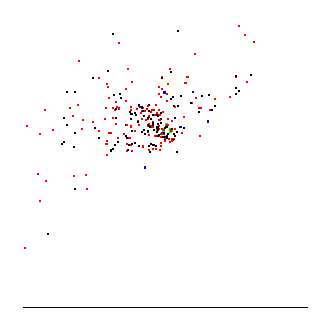
\includegraphics[width=0.3\linewidth]{img/bcn_nearest_top5_1less.eps} e)
          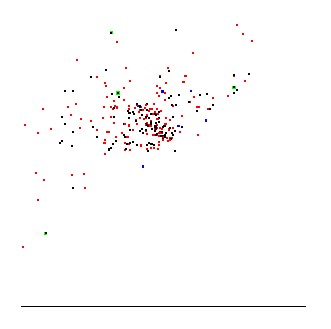
\includegraphics[width=0.3\linewidth]{img/bcn_farthest_all_1less.eps} f)
            \hspace{0.15\linewidth} Nearest \hspace{0.20\linewidth}  Top-$5$ nearest \hspace{0.20\linewidth}  Farthest
%          \includegraphics[width=0.3\linewidth]{img/bcn_area_2.eps} f)
          \caption{In red the hotels of Barcelona, in blue 9 (top) and 8 (bottom) query points, in green the obtained skyline hotels %from near a) and d), from near top-5 b) and e), from far c) and e)
          }\label{fig:bcn_region}
        \end{center}
     \end{figure}




\subsection{Performance analysis}\label{subsec:exp_res}

The experimental results have been obtained using an Intel Core i7-7700 CPU @3.6GHz with 32GB of RAM and a GPU Nvidia GTX 1060 6GB. Input data has been randomly generated using the standard C++ random library within a squared domain $[0,1]\times[0,1]$ and the weights have also been randomly generated within $[0,10]$. The sizes of $|P|$ vary from 2000 to 100K and $|Q|$ is fixed to 100.

In Figure~\ref{fig:rtimes} we present several information related to the performance of the sequential $WDS$ and the parallel $PWBF$ algorithms. In each chart there is information of 28 different settings corresponding to 14 different $|P|$. We considered two different distributions of $P$ and $Q$ for each cardinality, one leading to a small output (left edge and bar series) and the other to a small output (right edge and line series). The size of the obtained outputs for the nearest and farthest cases are represented in char a), note that generally, there exist more nearest than farthest spatial skyline points, but it is not always in this way. In the following rows we present the running times, speedups and number of computations done with each presented algorithm for the nearest case in the first column and the farthest in the second. In all the charts data related to WDS is colored purple and that to PWBF blue. Apart from presenting the running times in the second row, we also present the speedups of the PWBF with respect to the WDS algorithm in the third one. Finally in the last row we present the number of computations performed in each case. As it is expected, the PWBF algorithm does much more computations than the WSD algorithm, but since they are done in parallel, its running times are better than those of the WSD. In fact, the parallel PWBF algorithm notoriously outperforms the sequential WSD in all the cases except for the smallest case for the nearest case in which case the running times are almost the same. Hence, exploiting the parallel capabilities of the GPU is worthwhile and drives to a robust and fast algorithm.

    \begin{figure}[]
      \begin{center}
        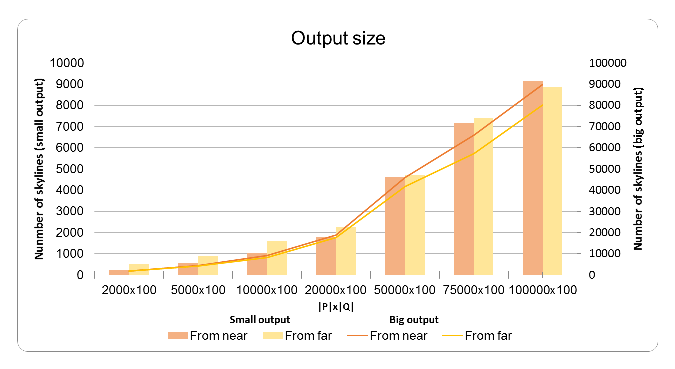
\includegraphics[width=0.45\linewidth]{img/osize_nf_sb.eps}a) \\
        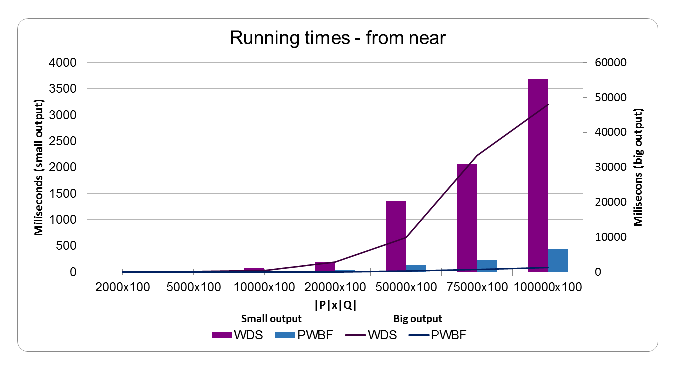
\includegraphics[width=0.45\linewidth]{img/rt_n_sb.eps} b)
        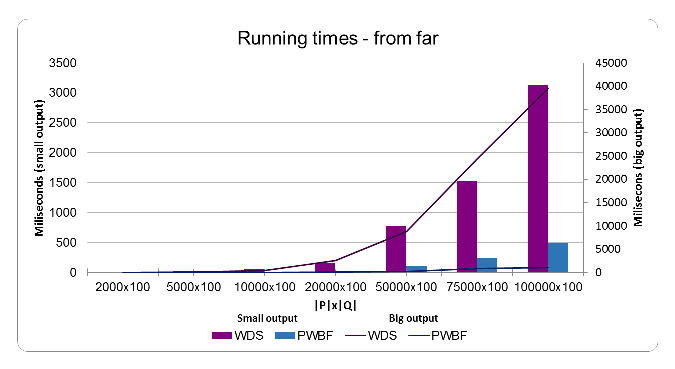
\includegraphics[width=0.45\linewidth]{img/rt_f_sb.eps} c)
        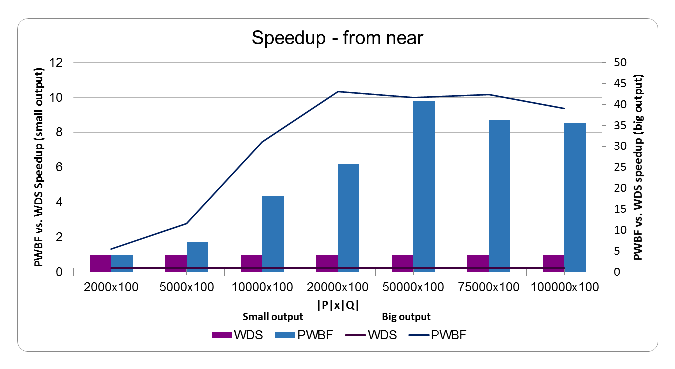
\includegraphics[width=0.45\linewidth]{img/sp_n_sb.eps} d)
        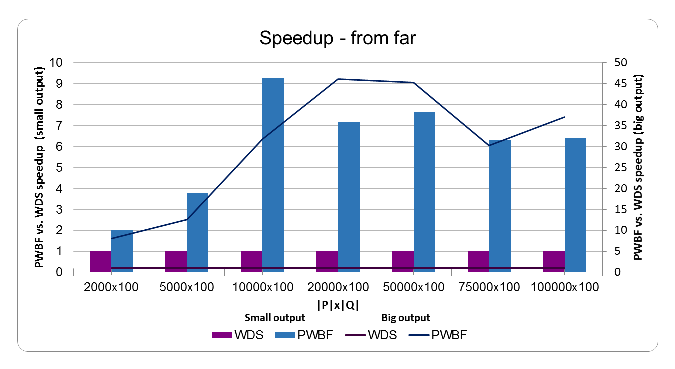
\includegraphics[width=0.45\linewidth]{img/sp_f_sb.eps} e)
        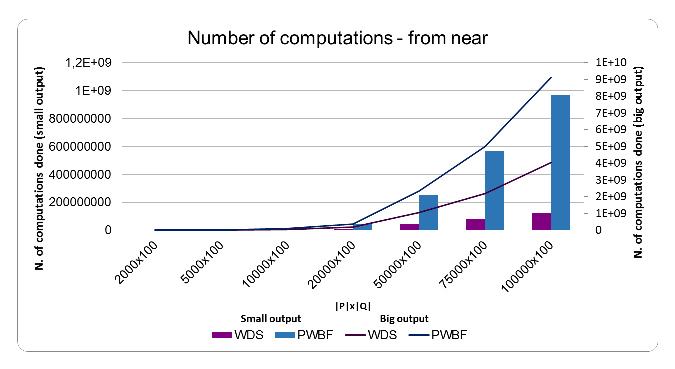
\includegraphics[width=0.45\linewidth]{img/comp_n_sb.eps} f)
        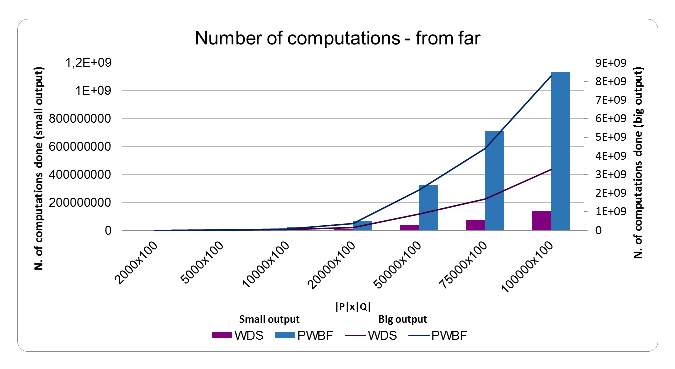
\includegraphics[width=0.45\linewidth]{img/comp_f_sb.eps} g)
        %
\includegraphics[width=0.3\linewidth]{img/P3_q2.eps}
        \caption{a) Output size. Running times of WDS and PWBF from: b) near c) far. Speedup of PWBF vs. WDS from: d) near, e) far. Number of computations done from: f) near, g) far}\label{fig:rtimes}
        %c) The Voronoi region of $p_j$ intersects with $CH(Q)$ and $p_j$ dominates from far $p_i$.
      \end{center}
    \end{figure}

Finally, we want to mention that extracting the top$-k$ skylines, independently of whether it is done a posteriorly or directly form the beginning, does not produce important changes on the running times. In fact, the most important delay do not exceed 60 milliseconds which makes that there were no differences between the graphics obtained with this running times and speedups for the top-k problem and those presented in Figure~\ref{fig:rtimes}.


\subsection{Discarded algorithms}\label{sec:ExpResultsDis}

Apart from the algorithms presented in detail in the paper, we have also experimented with other potential algorithms. We accurately designed, implemented and tested them but we did not report them in detail in the paper because they performed worse than the presented ones. Among these algorithms we want to remark the following ones:\\


\noindent {\it WDS Parallel version:} We implemented a parallel version of the WDS algorithm by using a standard reduce technique. \iffalse Even though, the implementation has been done accurately taking all the advantages of the parallel capabilities of the GPU,\fi  The obtained running times are better than those obtained with the sequential WDS but worst than those obtained with the PWBF. \\% (see figure~\ref{fig:other_rt}).\\(PWDS)

\noindent {\it PWBF parallelized in the CPU:} We implemented a multi-CPU-thread version of the PWBF algorithm. This implementation works better than the WDS algorithm but worse than PWBF that runs in a single-GPU.\\ % We think that a single-GPU algorithm has to be compared with the best single-CPU algorithm to solve the problem. \\(cpuPWBF)

\noindent {\it PWBF using one thread per pair:} when parallelizing the brute force algorithm one can consider $|P|(|P|-1)$ threads, one thread per pair $(p_i,p_j) \in P\times P$ with $i\neq j$. Each thread considers the pair and checks wether $p_i$ dominates $p_j$ by analysing the $|Q|$ queries. The amount of work done by each thread is smaller than that done in PWBF, this makes that the compute capabilities of the GPU were not completely exploited. Moreover, the number of threads needed is greater. Among all, even though this algorithm had always faster running times than WDS, they were always slower than those of PWBF.\\%(P2WBF)


\noindent {\it PWBF* once per pair:} The PWBF algorithm and all its the mentioned versions consider each pair $p_i,p_j$ twice, once to check whether $p_i$ dominates $p_j$ and twice to check whether $p_j$ dominates $p_i$. Consequently, some of the work is done twice, we tried to avoid it by adapting the algorithms to answer both queries at the same time. This is done by initializing the points of $P$ as non-dominated and considering only pairs with $i<j$. Then, when a weighted point is dominated it is marked as dominated. The running times of the PWBF algorithm increased, probably because of the extra time needed to initialize all the points as non-dominated. On the contrary, the running times of the other implemented versions of the PWBF algorithms improved, but were still greater than the running times of the PWBF algorithm.\\ %(PWBF1p*)

%Hence, after designing, implementing and testing all these algorithms the best sequential algorithm is the WSD and the parallel one the PWBF.


%
% \begin{figure}[]
%      \begin{center}
%        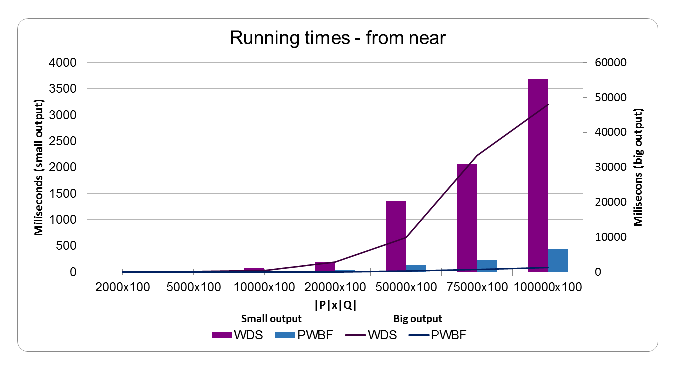
\includegraphics[width=0.45\linewidth]{img/rt_n_sb.eps} a)
%        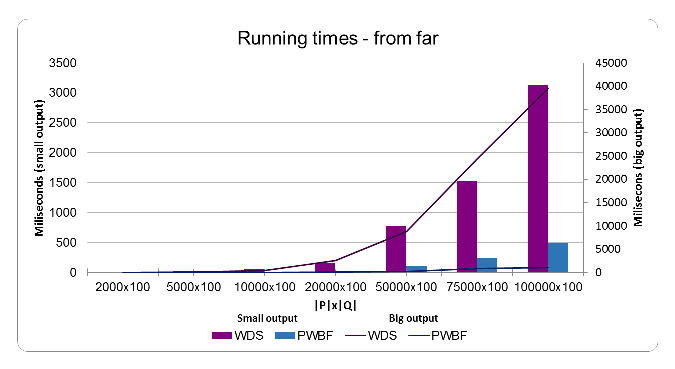
\includegraphics[width=0.45\linewidth]{img/rt_f_sb.eps} b)
%        \includegraphics[width=0.45\linewidth]{img/sp_n_sb.eps} c)
%        \includegraphics[width=0.45\linewidth]{img/sp_f_sb.eps} d)
%        \includegraphics[width=0.45\linewidth]{img/comp_n_sb.eps} e)
%        \includegraphics[width=0.45\linewidth]{img/comp_f_sb.eps} f)
%        %\includegraphics[width=0.3\linewidth]{img/P3_q2.eps}
%        \caption{Running times (top) and speedup of $PBF$ vs. $WDS$ (bottom) for the nearest (left) and farthest (right) case}\label{fig:rtimes} \textcolor{red}{falta indicar que les linies son small i les barres big a la llegenda}\label{fig:other_rt}
%        %c) The Voronoi region of $p_j$ intersects with $CH(Q)$ and $p_j$ dominates from far $p_i$.
%      \end{center}
%    \end{figure}





\section{Conclusions} \label{sec:Conclusions}

We have presented, theoretically studied and sequentially and parallelly solved the spatial skyline problem under the weighted Euclidean distance for the first time. We have proven that most of the properties of the traditional spatial skyline problems are no longer true under the weighted Euclidean distance, which does not fulfill the triangular inequality. The from near, from far and top-$k$ versions of the problem have been analyzed.

Two fast and robust algorithms to solve the problem have been presented in detail, one runs sequentially in the CPU (WSD) and the other exploits the parallel capabilities of the GPU (PWBF). These algorithms have been analyzed and compared theoretically and experimentally. The parallel algorithm outperforms the sequential one by a factor between 6 and 10 in most of the analyzed settings as it was predicted by the theoretical complexity analysis comparison. We have also compared these two algorithms with several other sketched and implemented algorithms that can be used to solve the problem and that have been discarded to be slower.

We also developed an interface to work with the problem that allows to easily visualize the obtained solution and to store it in a {\it .json} or {\it binary} file. Since the obtained solution sometimes still has too much candidates, we allow the user to obtain the top-$k$ spatial skylines according to a scoring function that can be selected among four predefined once. However, the scoring function could easily be defined by the user meanwhile it only depends on the distances from the skyline to the query points. We allow the user to first obtain the skylines and then identify the top$-k$ among them, or to directly determine only the top-$k$ ones.


\section{Acknowledgments}
This work has been partially funded by the {\it Ajut per la millora de la productivitat científica}/UdG/3/Ref. MPCUdG2016-031UdG-52211-C2-2-R.
%We would also like to acknowledge the NVIDIA Corporation for their donation of the Tesla K40 GPU.

\begin{thebibliography}{100}


\bibitem{AE84}
Aurenhammer,~F., Edelsbrunner,~H.  An optimal algorithm for constructing the weighted
voronoi diagram in the plane. Pattern Recognition, 17(2) (1984) 251–-257.

\bibitem{BGZ04} W.T. Balke, U. G\"untzer, J.X. Zheng, \emph{Efficient distributed skylining for web information systems}:
Proceedings of EBT, 2004.

\bibitem{BBCDKS10}
Bhattacharya,~B., Bishnu,~A., Cheong,~W., Das,~S., Karmakar,~A., Snoeyink,~J., 2010. Computation of non-dominated points using Voronoi diagrams compact, in: Walcom: Algorithms and Computation, Proceedings, LNCS, 5942, 82--93.

\bibitem{BS97}
B.~Boots, R.~South, Modeling retail trade areas using
higher-order, multiplicatively weighted {V}oronoi diagrams,
Journal of Retailing 73(3) (1997) 519--536.

\bibitem{BKS01} Borzsony,~S., Kossmann,~D., Stocker,~K., 2001. The Skyline Operator, in: Proceedings of the 17th International Conference on Data Engineering, 421--430.

\bibitem{CLY12} Choi,~W., Liu,~L., Yu,~B., 2012. Multi-criteria decision making With skyline computation,
in: 13th International Conference on Information Reuse and Integration, IEEE, 316--323.


\bibitem{DS07} Dellis,~E., Seeger,~B., 2007. Efficient computation of reverse skyline queries, in:
Proceedings of the 33rd International Conference on Very large data bases (VLDB '07), 291--302.

\bibitem{Dre94}
T.~Drezner, 1994. Optimal continuous location of a retail
facility, facility attractiveness, and market share: An
interactive model. Journal of Retailing. 70(1), 49--64.

\bibitem{DD02}
T.~Drezner, Z.~Drezner, 2002. Validating the Gravity-Based
Competitive Location Model Using Inferred Attractiveness. Annals
OR 111(1-4), 227--237.

\bibitem{FS13}
M.~Fort and J.A.~Sellar\`es, \emph{Finding influential location regions based on reverse k-neighbor queries}, Knowledge-Based Systems, Volume 47 (2013)  pp.~35-52.

\bibitem{FS14a}
M.~Fort and J.A.~Sellar\`es, \emph{Solving the k-influence region problem with the GPU},
Information Sciences, \textbf{269} (2014) 255--269.

\bibitem{FS15}
M.~Fort and J.A.~Sellar\`es, \emph{Common influence region problems},  Information Sciences, \textbf{321} (2015) 116--135.

\bibitem{FS16}
M.~Fort and J.A.~Sellar\`es, \emph{Efficient multiple bichromatic mutual nearest neighbor query processing}, Information Systems, \textbf{62} (2016) 136--154.


\bibitem{FS16b}
M.~Fort and J.A.~Sellar\`es
\emph{Solving multiple kth smallest dissimilarity queries for non-metric dissimilarities with the GPU},
Information Sciences, Volumes 361-362 (2016) pp.~66-83.

\bibitem{GLZ14} Gao,~Y., Liu,~Q., Zheng,~B., Chen,~G., 2014. On reverse skyline efficient query processing, Expert Systems with Applications, 41 (7), 3237--3249.

\bibitem{GLCCL15}
Y.~Gao, Q.~Liu, L.~Chen, G.~Chen, Q.~Li
\emph{Efficient algorithms for finding the most desirable skyline objects}, Knowledge-Based Systems, \textbf{89} (2015) 250-264.


\bibitem{GSG07} Godfrey,~P., Shipley,~R., Gryz,~L., 2007. Algorithms and analyzes for maximal vector computation, The VLDB Journal, 16 (1), 5--28.

\bibitem{KTM17} Kalyvas,~C., Tzouramanis,~T., Manolopoulos And Processing 2017. Temporal Databases Skyline
Queries in, in: Proceedings of the Symposium on Applied Computing (SAC '17), ACM, New York, 893--899.

\bibitem{KRR02} Kossmann,~D., Ramsak,~F., Rost,~S., 2002. Shooting stars in the sky: An online algorithm
for skyline queries, in: Proceedings of the 28th International Conference on Very Large Data Bases (VLDB '02 ), 275--286.

\bibitem{KLP75} Kung,~H.-T., Luccio,~F. Preparata,~FP, 1975. On finding the maximum of a set of vectors, Journal of the ACM, 22 (4), 469--476.

\bibitem{LSAH11}
M.~Lee, W.~Son, H.~Ahn, and S.~Hwang, \emph{Spatial skyline queries: exact and
approximation algorithms}, GeoInformatica (2011) 15(4), 665--697.

\bibitem{LPYL11} Li,~Z. Peng,~Z. Yan,~J., Li,~T., 2011. Continuous dynamic skyline queries over data
stream, Journal of Computer Research and Development, 48 (1), 77--85.

\bibitem{LZZ13} Lin,~Q., Zhang,~Y., Zhang,~W., Li,~A., 2013. General Efficient computation space skyline,
World Wide Web, 16 (3), 247--270.

\bibitem{MT04}
B.~Mendes, I.H.~Themido
\emph{Multi-outlet retail site location assessment},
International Transactions in Operational Research 11 (1) (2004), 1--18.

\bibitem{MPLZ14} Mullesgaard,~K., Pedersen,~JL, Lu,~H., Zhou,~Y., 2014. Efficient Computation Skyline in
MapReduce, in: Proceedings of 17th International Conference on Extending Databases Technology (EDBT), 37--48.

\bibitem{OpenStreetMap} \emph{OpenStreetMap}, https://www.openstreetmap.org, last accesed at 20 july 2008.

\bibitem{PTFS05} Papadias,~D., Tao,~Y., Fu,~G., Seeger,~ B., 2005. Progressive skyline computation in
database systems, ACM Transactions on Database Systems, 30 (1), 41--82.

\bibitem{PMS13} Park,~Y., Min,~J.-K., Shim,~K., 2013. Parallel computation of skyline and reverse skyline
queries using mapreduce, Proceedings of the VLDB Endowment, 6 (14), 2002--2013.

\bibitem{PS14} Prema Steffi, R., Sundaramoorthy, S. \emph{Top-K Spatial Preference Query
with Range Based Skyline Query in Mobile Environment}, International Journal
of Computer Science International Journal of Computer Science and Engine
and Engineering, 2(3), 2014, pp.~46--50.

\bibitem{SS06} M.~Sharifzadeh, and C.~Shahabi, The Spatial Skyline Queries. Proceedings of the 32nd
International Conference on Very Large Data Bases (VLDB '06), 2006, pp.~751--762.

\bibitem{SSK09}
M.~Sharifzadeh, C.~Shahabi, and L.~Kazemi, \emph{Processing spatial skyline queries in both vector spaces and spatial network databases}, ACM Trans. Database Syst. \textbf{34(3)} (2009), pp.~1--45.

\bibitem{SHA14}
W. Son, S.W. Hwang, H.K. Ahn, \emph{MSSQ: Manhattan Spatial Skyline Queries}, Inf. Syst. 40, 2014, pp.~67--83.

\bibitem{SSKA17} W.~Son, F.~Stehn, C.~Knauer, H.K.~Ahn, \emph{Top-k Manhattan spatial skyline queries},
Information Processing Letters.  \textbf{123} (2017),  pp.~27--35.

\bibitem{SB13} Soudani,~NM, Baraani-Dastgerdi,~A., 2011. The Spatial Nearest Neighbor Skyline Queries,
International Journal of Database Management Systems, 3 (4), 65--79.

\bibitem{TXP07} Tao,~Y., Xiao,~X., Pei,~J., \emph{Efficient skyline and top-k retrieval in subspaces}, IEEE Transactions on Knowledge and Data Engineering, 19 (8), (2007) 1072--1088.

\bibitem{WZSK17} W.~Wang, ~J.~Zhang,~M.T.~Sun, and~W.S.~Ku, \emph{Efficient Parallel Spatial skyline
Evaluation using MapReduce}, 2oth International Coferecne on Extending Database Technology (EDBT'17) (2017), pp.~426--437.

\bibitem{XW18}
T.~Xu, G.~Wang
\emph{Finding strongly connected components of simple digraphs based on generalized rough sets theory},
Knowledge-Based Systems, Volume 149 (2018) pp.~88-98.

\bibitem{XZCMW18}
K.~Xu, X.~Zheng, Y.~Cai, H.~Min, T.~Wong
\emph{Improving user recommendation by extracting social topics and interest topics of users in uni-directional social networks}, Knowledge-Based Systems, Volume 140 (2018) pp.~120-133.

\bibitem{YLIH13}
G-W. You, M-W. Lee, H. Im,S-W. Hwang, \emph{The Farthest Spatial Skyline Queries}, Inf. Syst. 38 (2013) pp.~286--301.
% ------- BIB PT --------- REUBICAR ----------

%\textcolor{red}{Comenca la del projecte de tesi, no esta ordenada i esta en un format diferent}

\end{thebibliography}

\end{document}


\bibliographystyle{amsplain}

\begin{thebibliography}{00}

\bibitem{AKSU12} Afrati, F.N., Koutris, P., Suciu, D., Ullman, J.D,  \emph{Parallel
skyline queries}, Proc. ICDT, 2012, pp.~274--284.

\bibitem{BAM13} Bogh, K.S., Assent, I., Magnani, M. Efficient, \emph{GPU-based skyline
computation}, Proc. DaMoN, 2013, pp.~X--Y.

\bibitem{BCP08}	I. Bartolini, P. Ciaccia, M. Patella, \emph{Efficient sort-based skyline evaluation},
ACM Trans. Database Syst.33(4), 2008, pp.~1--49.

\bibitem{BEKMRZZ13} T. Bernecker, T. Emrich, H.P. Kriegel, N. Mamoulis, M. Renz, S. Zhang, A. Züfle, \emph{Spatial inverse query processing}, GeoInformatica 17(3), 2013, pp.~449--487.

\bibitem{BKS01} S.~B\"orzs\"onyi, D.~Kossmann, and K.~Stocker, \emph{The skyline operator},
Data Engineering, 2001. Proceedings. 17th International Conference on, 2001, pp.~421--430.

\bibitem{CCM13} J. Chomicki, P. Ciaccia, N. Meneghetti, \emph{Skyline queries, front and
back}, SIGMOD Record 42(3), 2013, pp.~6--18.

\bibitem{CJTTZ06} C.Y. Chan, H.V. Jagadish, K.L. Tan, A.K.H. Tung, Z.
Zhang,\emph{Finding k-dominant skylines in high dimensional
space}, SIGMOD Conference, 2006, pp.~503--514.

\bibitem{CL09} L. Chen and X. Lian. \emph{Efficient processing of metric skyline
queries}, IEEE Trans. on Knowl. and Data Eng., 21(3), 2009,
pp.~351--365.

\bibitem{CLY12} W. Choi, L. Liu, and B. Yu, \emph{Multi-criteria decision making
with skyline computation}, IEEE Information Reuse and Integration,
2012, pp.~316--323.

\bibitem{CSL13} Y.C. Chung, I.F. Su, C. Lee, \emph{Efficient computation of
combinatorial skyline queries} Inf. Syst. 38(3), 2013,
pp.~369--387.

\bibitem{DS07} E. Dellis and B. Seeger, \emph{Efficient computation of reverse
skyline queries}, Proc. 33rd Inter. Conf. on Very Large Data
Bases, 2007, pp.~291--302.

\bibitem{FGJCML13} X. Feng, Y. Gao, T. Jiang, L. Chen, X. Miao and Q. Liu
\emph{Parallel k-Skyband Computation on Multicore Architecture},
APWeb 2013, LNCS vol. 7808, 2013, pp.~827--837.

\bibitem{FJZ09} D. Fuhry, R. Jin, D, Zhang, \emph{Efficient skyline computation in
metric space}, EDBT, 2009, pp.~1042--1051.

\bibitem{GMHS13} Y. Gae-won,  L. Mu-Woong, I. Hyeonseung, H. Seung-won, \emph{The arthest spatial skyline queries}, Information Systems \textbf{38} (2013), pp. 286--301.

\bibitem{GSG07} P.~Godfrey, R.~Shipley, and J.~Gryz, \emph{Algorithms and analyses for
maximal vector computation}, The VLDB Journal \textbf{16} (2007), pp.~5--28.

\bibitem{GXI12} X. Guo, C. Xiao, Y. Ishikawa, \emph{Combination Skyline Queries}, LNCS
Vol. 7600, 2012, pp.~1--30.

\bibitem{HLKP10} A. Han, Z. Li, D. Kwon, and Y. Park, \emph{An Efficient Method for
Processing Reverse Skyline Queries over Arbitrary Spatial
Objects}, Proc. of Database Technology and Applications, 2010,
pp.~1--4.

\bibitem{HLKP14} A. Han, Z. Li, D. Kwon, and Y. Park, \emph{An Efficient Pruning
Method to Process Reverse Skyline Queries}, Journal of Information
Science and Engineering, Vol. 30 No. 2, 2014, pp.~XXX–-YYY.

\bibitem{HPP11} H. Im, J. Park, S. Park, \emph{Parallel skyline
computation on multicore architectures}, Inf. Syst. 36(4), 2011,
pp.~808--823.

\bibitem{HP12} H. Im, S. Park, \emph{Group skyline computation}, Inf. Sci.
Vol. 188, 2012, pp.~151--169.

\bibitem{JTEH07} W. Jin, A.K.H. Tung, M. Ester, J. Han, \emph{On Efficient
Processing of Subspace Skyline Queries on High Dimensional Data},
SSDBM, 2007, pp.~X--Y.

\bibitem{KLH09}  J. Kim, J. Lee, S.W. Hwang, \emph{Skyline View: Efficient Distributed Subspace Skyline Computation},
DaWaK'09, 2009, pp.~312--324.

\bibitem{KYZ11} K\"ohler, H., Yang, J., Zhou, X, \emph{Efficient parallel skyline
processing using hyperplane projections}, ISIGMOD Conference,
2011, pp.~85–-96.

\bibitem{LC08} X. Lian and L. Chen, \emph{Monochromatic and bichromatic reverse
skyline search over uncertain databases}, Proc. ACM SIGMOD Inter.
Conf. on Management of Data, 2008, pp.~213–-226.

\bibitem{LCH09} Z. Ling, L. Cuiping and C. Hong, \emph{Efficient computation of
reverse skyline on data stream}, Inter. Joint Conf. on
Computational Sciences and Optimization, 2009, pp.~735--739.

\bibitem{LGCLJ12} Liu, Q., Gao, Y., Chen, G., Li, Q., Jiang, T, \emph{On efficient
reverse k-skyband query processing}, DASFAA 2012, LNCS vol. 7238,
2012, pp.~544-–559.

\bibitem{LH14} J. Lee, S.W Hwang, \emph{Scalable skyline computation using a balanced pivot selection technique}, Inf. Syst. 39, 2014, pp.~1--21.

\bibitem{LLZLT10} K. C. K. Lee, W.C. Lee, B. Zheng, H. Li, Y. Tian, \emph{Z-SKY: an efficient skyline query processing framework based on Z-order}, VLDB J. 19(3), 2010, pp.~333--362.

\bibitem{LSAH11}
M.~Lee, W.~Son, H.~Ahn, and S.~Hwang, \emph{Spatial skyline queries: exact and
approximation algorithms}, GeoInformatica (2010).

\bibitem{LY09}
H. Lu, M-L. Yiu, \emph{Identifying the Most Endangered Objects from Spatial Datasets}, Proc. Scientific and Statistical Database Management SSDBM (2009) pp. 608--626

\bibitem{LY11} H. Lu, M.L. Yiu, \emph{On Computing Farthest Dominated Locations},
IEEE Transactions on Knowledge and Data Engineering, vol. 23, no. 6, 2011, pp.~928--941.

\bibitem{LPLSY10} J. Lim, Y. Park, J. Lee, D. Seo, and J. Yoo, \emph{An efficient
method for processing reverse skyline queries}, Proc. of Mobile
Congress, 2010, pp.~1--5.

\bibitem{LVDN14} S. Liknes, A. Vlachou, C. Doulkeridis and K. Nørvag,
\emph{APSkyline: Improved Skyline Computation for Multicore
Architectures}, DASFAA 2014, 2014, pp.~X--Y.

\bibitem{LZZL13} Q. Lin, Y. Zhang, W. Zhang and A. Li, \emph{Efficient general spatial
skyline operator}, World Wide Web 16(3), 2013, pp.~247--270.

\bibitem{MLW09} Man Leung Wong,
\emph{Parallel multi-objective evolutionary algorithms on graphics processing units}, GECCO'09, 2009, pp.~2515--2522.

 \bibitem{SSKA17} W. Son, F. Stehn, C. Knauer, H.K. Ahn, \emph{Top-k Manhattan spatial skyline queries},
        Information Processing Letters, 123, 2017,  pp.~27-35.

\bibitem{PTFS05} Papadias, D., Tao, Y., Fu, G., Seeger, B,  \emph{Progressive skyline
computation in database systems.}, ACM Trans. Database Syst.
30(1), 2005, pp.~41--82.

\bibitem{PS14} Prema Steffi, R., Sundaramoorthy, S. \emph{Top-K Spatial Preference Query
with Range Based Skyline Query in Mobile Environment}, International Journal
of Computer Science International Journal of Computer Science and Engine
and Engineering, 2(3), 2014, pp.~46--50.

\bibitem{SCL10} I.F. Su, Y.C. Chung, C. Lee, \emph{Top-k Combinatorial Skyline
Queries} DASFAA, 2010, pp.~79--93.

\bibitem{SHA14} W. Son, S.W. Hwang, H.K. Ahn, \emph{MSSQ: Manhattan Spatial Skyline Queries}, Inf. Syst. 40, 2014, pp.~67--83.

\bibitem{SL10} T. Skopal and J. Lokoc, \emph{Answering Metric Skyline Queries by
PM-tree}, Proc. Dateso, 2010, pp.~22--37.

\bibitem{SM12} A. Siddique, Y. Morimoto, \emph{Efficient k-dominant Skyline
Computation for High Dimensional Space with Domination Power
Index}, Journal of Computers, Vol 7(3), 2012, 608-615,
pp.~608--615.


\bibitem{VDK08} Vlachou, A., Doulkeridis, C., Kotidis, Y,  \emph{Angle-based space
partitioning for efficient parallel skyline computation},  Proc.
of SIGMOD, 2008, pp.~X--Y.

\bibitem{VN09} A. Vlachou, K. Nørvåg, \emph{Bandwidth-constrained distributed skyline computation}, MobiDE'09, 2009, pp.~17--24.

\bibitem{WAT13} Woods, L., Alonso, G., Teubner, J., \emph{Parallel computation of
skyline queries}, Proc. of FCCM, 2013, pp.~X--Y.

\bibitem{ZMC09} S. Zhang, N. Mamoulis, D.W. Cheung, \emph{Scalable skyline computation using object-based space partitioning} SIGMOD'09, 2009, pp.~483--494.

\bibitem{YLIH13} G-W. You, M-W. Lee, H. Im,S-W. Hwang, \emph{The Farthest Spatial Skyline Queries}
 Inf. Syst. 38, 2013, pp.~286--301.

\bibitem{YM09} M.L. Yiu, N. Mamoulis, \emph{Multi-dimensional top-k dominating queries}, VLDB J. 18(3), 2009, pp.~695--718.

\end{thebibliography}

